\documentclass{article}


\usepackage[nottoc,numbib]{tocbibind}
\usepackage[utf8]{inputenc}
\usepackage{graphicx}
\usepackage{subcaption}
\usepackage{geometry}
\usepackage{amssymb}
\usepackage{caption}
\usepackage{float}
\usepackage{wrapfig}
\usepackage{romannum}
\usepackage{physics}
\usepackage{amsmath,amsfonts,amsthm,bm} % Math packages
\geometry{margin=1in}

\errorcontextlines 10000
\begin{document}
\pagenumbering{gobble}
\begin{titlepage}
    \begin{center}
        \vspace*{1cm}
        \Large

\includegraphics[width=.4\linewidth]{../logo.pdf}\\
        \Large
\vspace{1cm}
        Machine Learning Practicum\\
        \huge
        \textbf{Classifying star spectra\\}
\Large  
        \vspace{1cm}
        \textbf{Andrej Kolar - Po{\v z}un\\}
        \vspace{0.8cm}

\vfill
\normalsize
\end{center}. 
\end{titlepage}
\newpage
\pagenumbering{arabic}
\section*{Intro}
Classifying different types of stars is a challenge in astronomy because of the seemingly limited amount of information that we have at our disposal - stars are so far, that they are effectively point sources of light. For this reason we consider the spectra of that light, which can give us a number of useful information about a star including its temperature, element composition, gravitational acceleration on the star's surface, angular velocity of the speed, magnetic field... It should be mentioned that while it's known that this information is contained in the spectra, obtaining it is a whole different problem - the physical laws governing all the involved components, such as the magnetohydrodynamics are immensly complicated. For that reason, we opt for an easier approach.
What adds to the challenge is also the fact that spectra can be altered as they pass the interstellar medium as well as the Earth's atmosphere.

\section*{Data}
We use the data set from the GALAH project, which is a scan of the sky performed by a telescope in Australia.
The spectra are normalised and the Doppler effect for frequency shifting is already accounted for. Very few (Probably especially nearby) stars are labelled among 7 categories.
Our goal is to categorize also the rest into one of those classes:
\begin{itemize}
\item MAB - Stars with molecular absorbtion lines
\item BIN - Binary stars
\item TRI - Triple stars
\item HFR - Hot, fast rotating stars
\item HAE - Stars with $H\alpha$ emissions
\item CMP - cold stars with few metals
\item DIB - hot stars with stronger interstellar absrobtions
\end{itemize}

The labelled data is small in size - only about 6 spectra per label. These can all be seen on Figure \ref{fig:labeled}, where for each class, about 6 different star (differing by color of the plot) spectra are shown.
We can see the classification task might be difficult. Some stars from different categories (such as CMP and BIN) seem to have pretty similar spectra. On the other hand the spectra appearing in the HAE category can have a variety of different shapes.
\begin{figure}[H]
\centering
\begin{subfigure}{.7\textwidth}
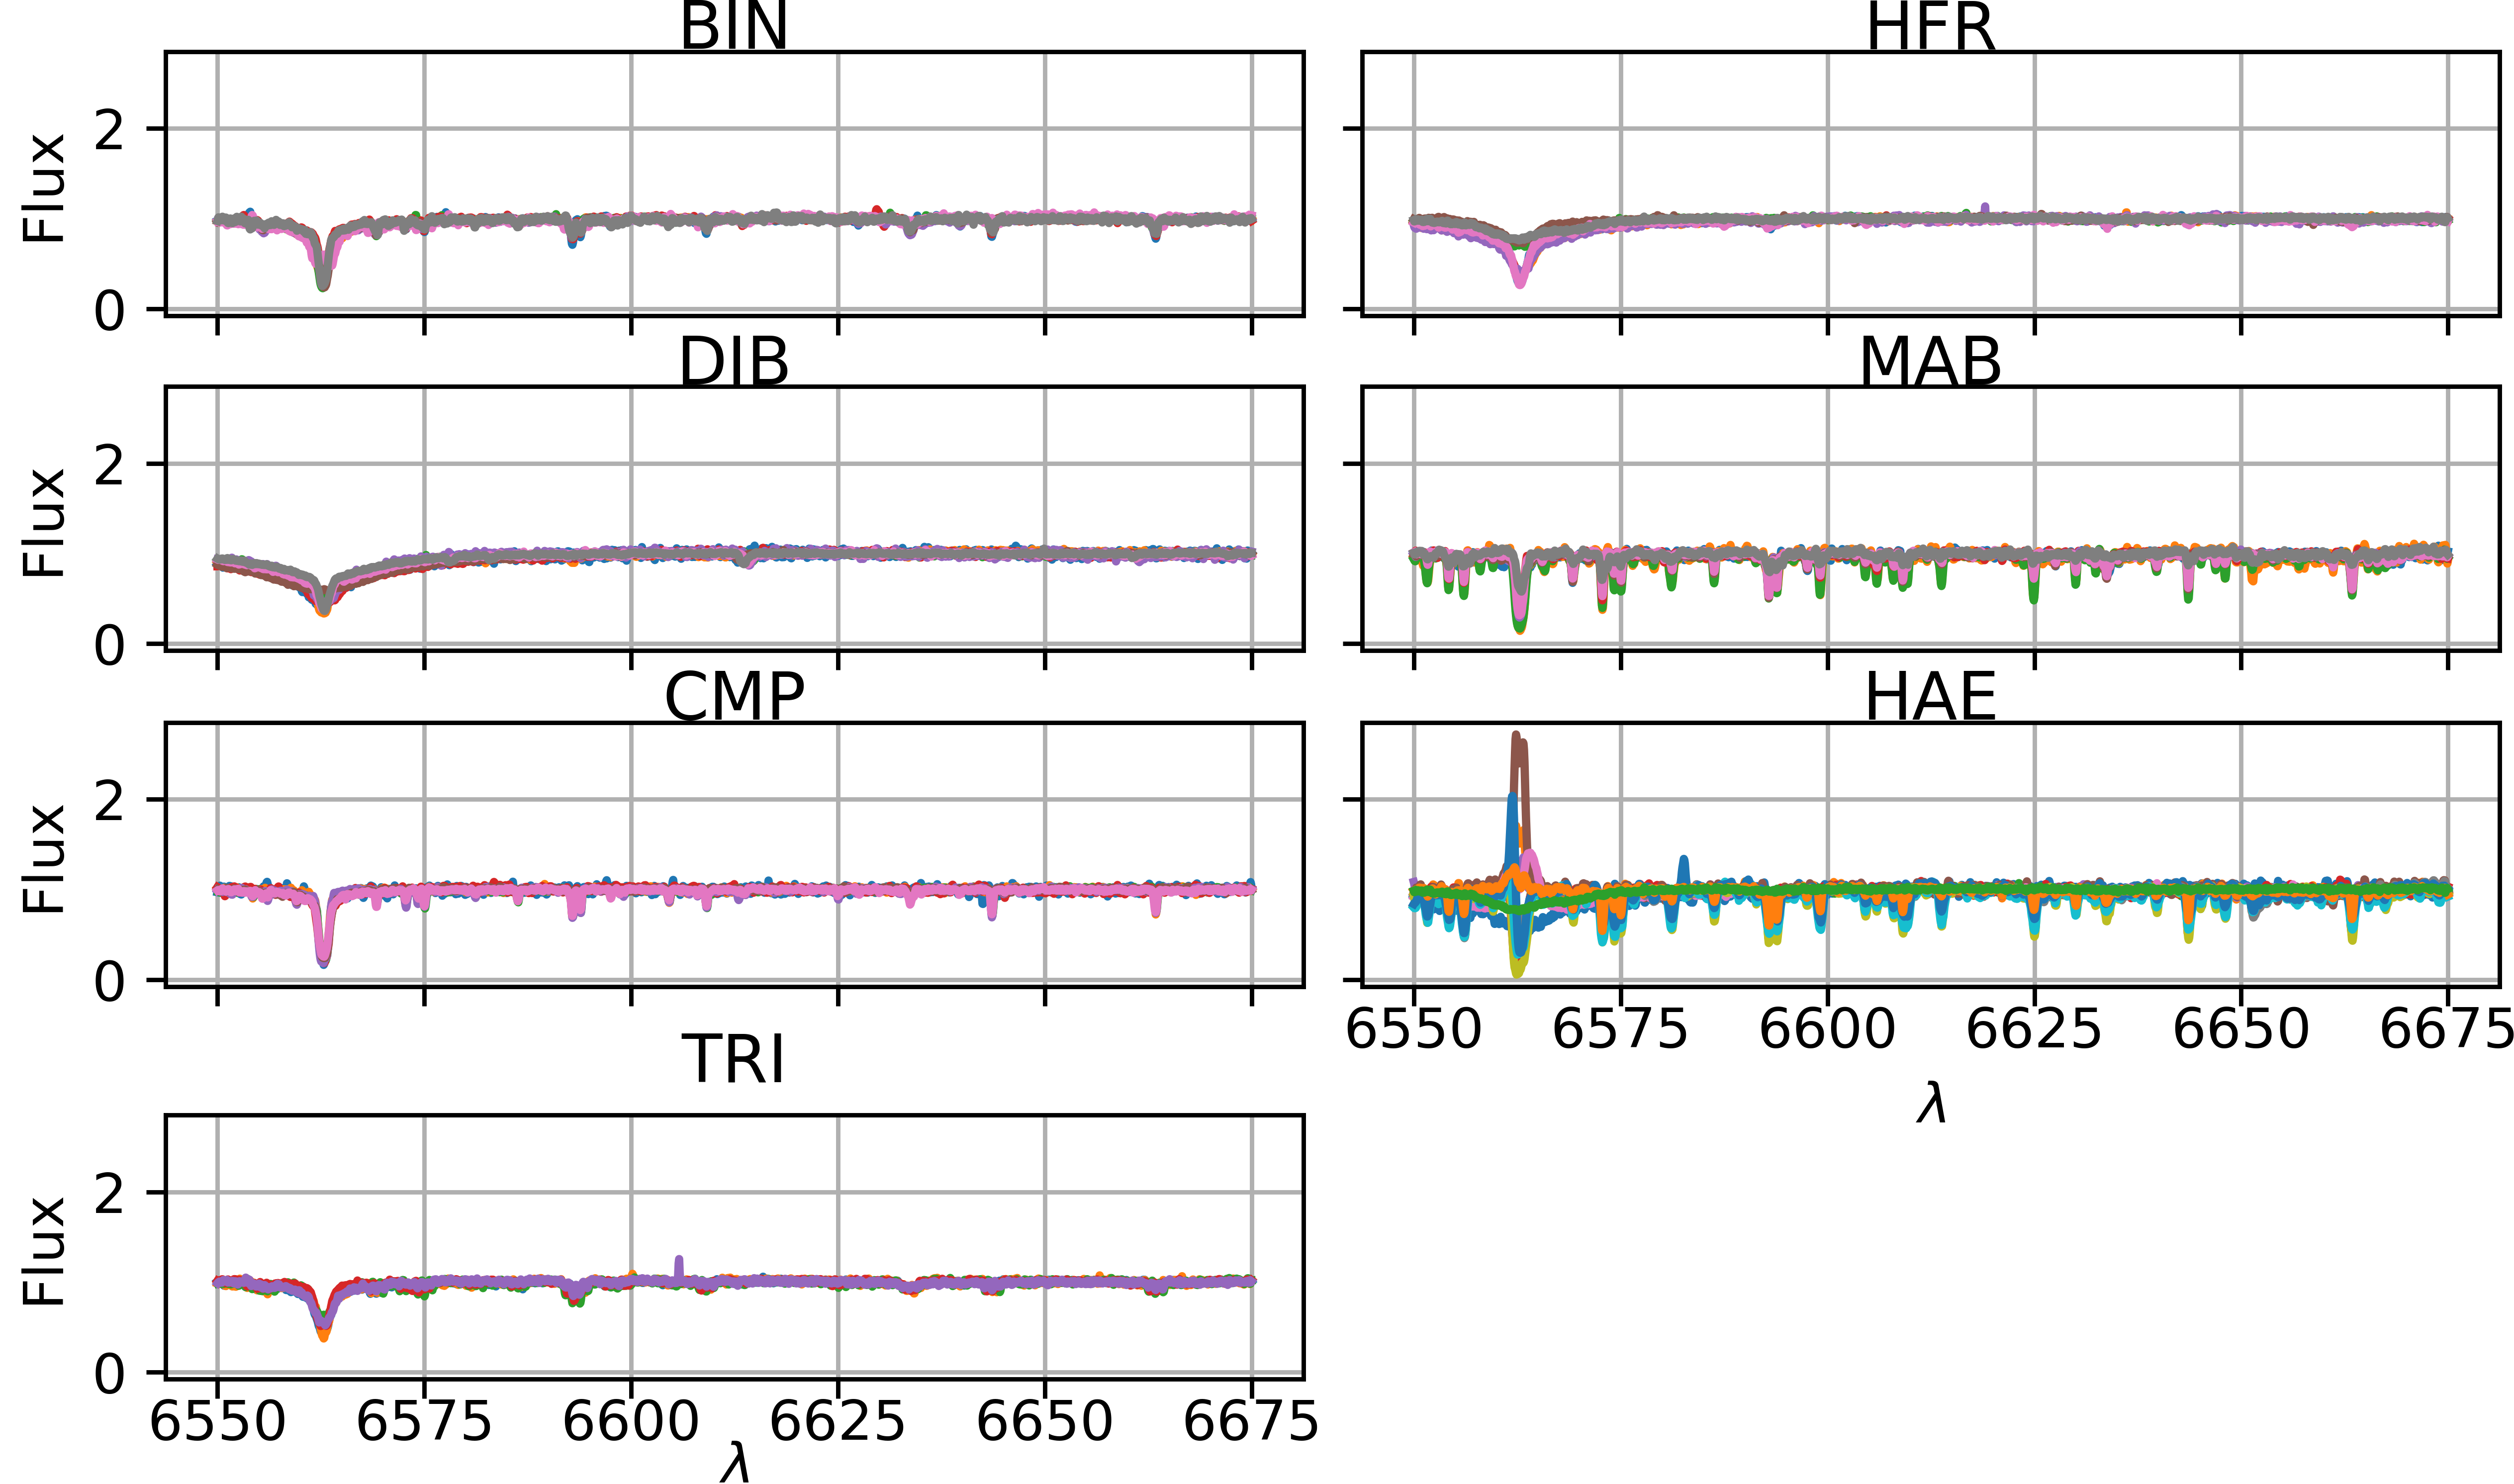
\includegraphics[width=\linewidth]{plots/labeled.png}
\end{subfigure}
\caption{Normalised flux values with respect to the wavelength (in Angstrom).}
\label{fig:labeled}
\end{figure}

\section*{Plan Overview}
We will employ some sort of classification algorithms to solve this problem. This means we assume that the labeled data are all possible classes in the dataset (which is perhaps unrealistic - would need an expert opinion). If that was not the case we would do better to perform clustering instead, leaving the number of clusters a variable.
Firstly, the numerical values of the wavelength are irrelevant, as they are the same for each spectra, so we cannot hope to distinguish them by this. For our purposes, the x-axis might as well be $1,2,3,\dots$. In fact, each of our spectra is defined by 2084 values (corresponding to the normalised flux value at the wavelength $i, i \in [1,2,\dots,2084]$.
What this means is that we effectively have date in a 2084 dimensional space, that we need to classify.

Clearly this amount of dimensions is too much so our first step is to perform a dimensionality reduction process, where it will hopefully be possible to classify the data.

\section*{Dimensionality reduction}
We start by probably the most well known method - Principal Component Analysis (PCA), which essentially forms a covariance matrix of our data, and diagonalizes it. In this way we get the principal directions (eigenvectors that correspond to highest eigenvalues), that correspond to the biggest variances in our data. In practice this is computed with SVD, but we will not delve into the implementation details (just use sklearn).
 
Either way, we first standarize the data (while the fluxes are already normalised in some sense, their mean is not 0, for example) and PCA project it to a lower dimensional space. The results can be seen on Figure \ref{fig:PCA2D}. The 2D projection is not satisfactory - the HAE data is all over the place and not very well seperated from other types. Similar issue happens in a 3D case (although difficult see on the below non-interactive image). 
\begin{figure}[H]
\centering
\begin{subfigure}{.48\textwidth}
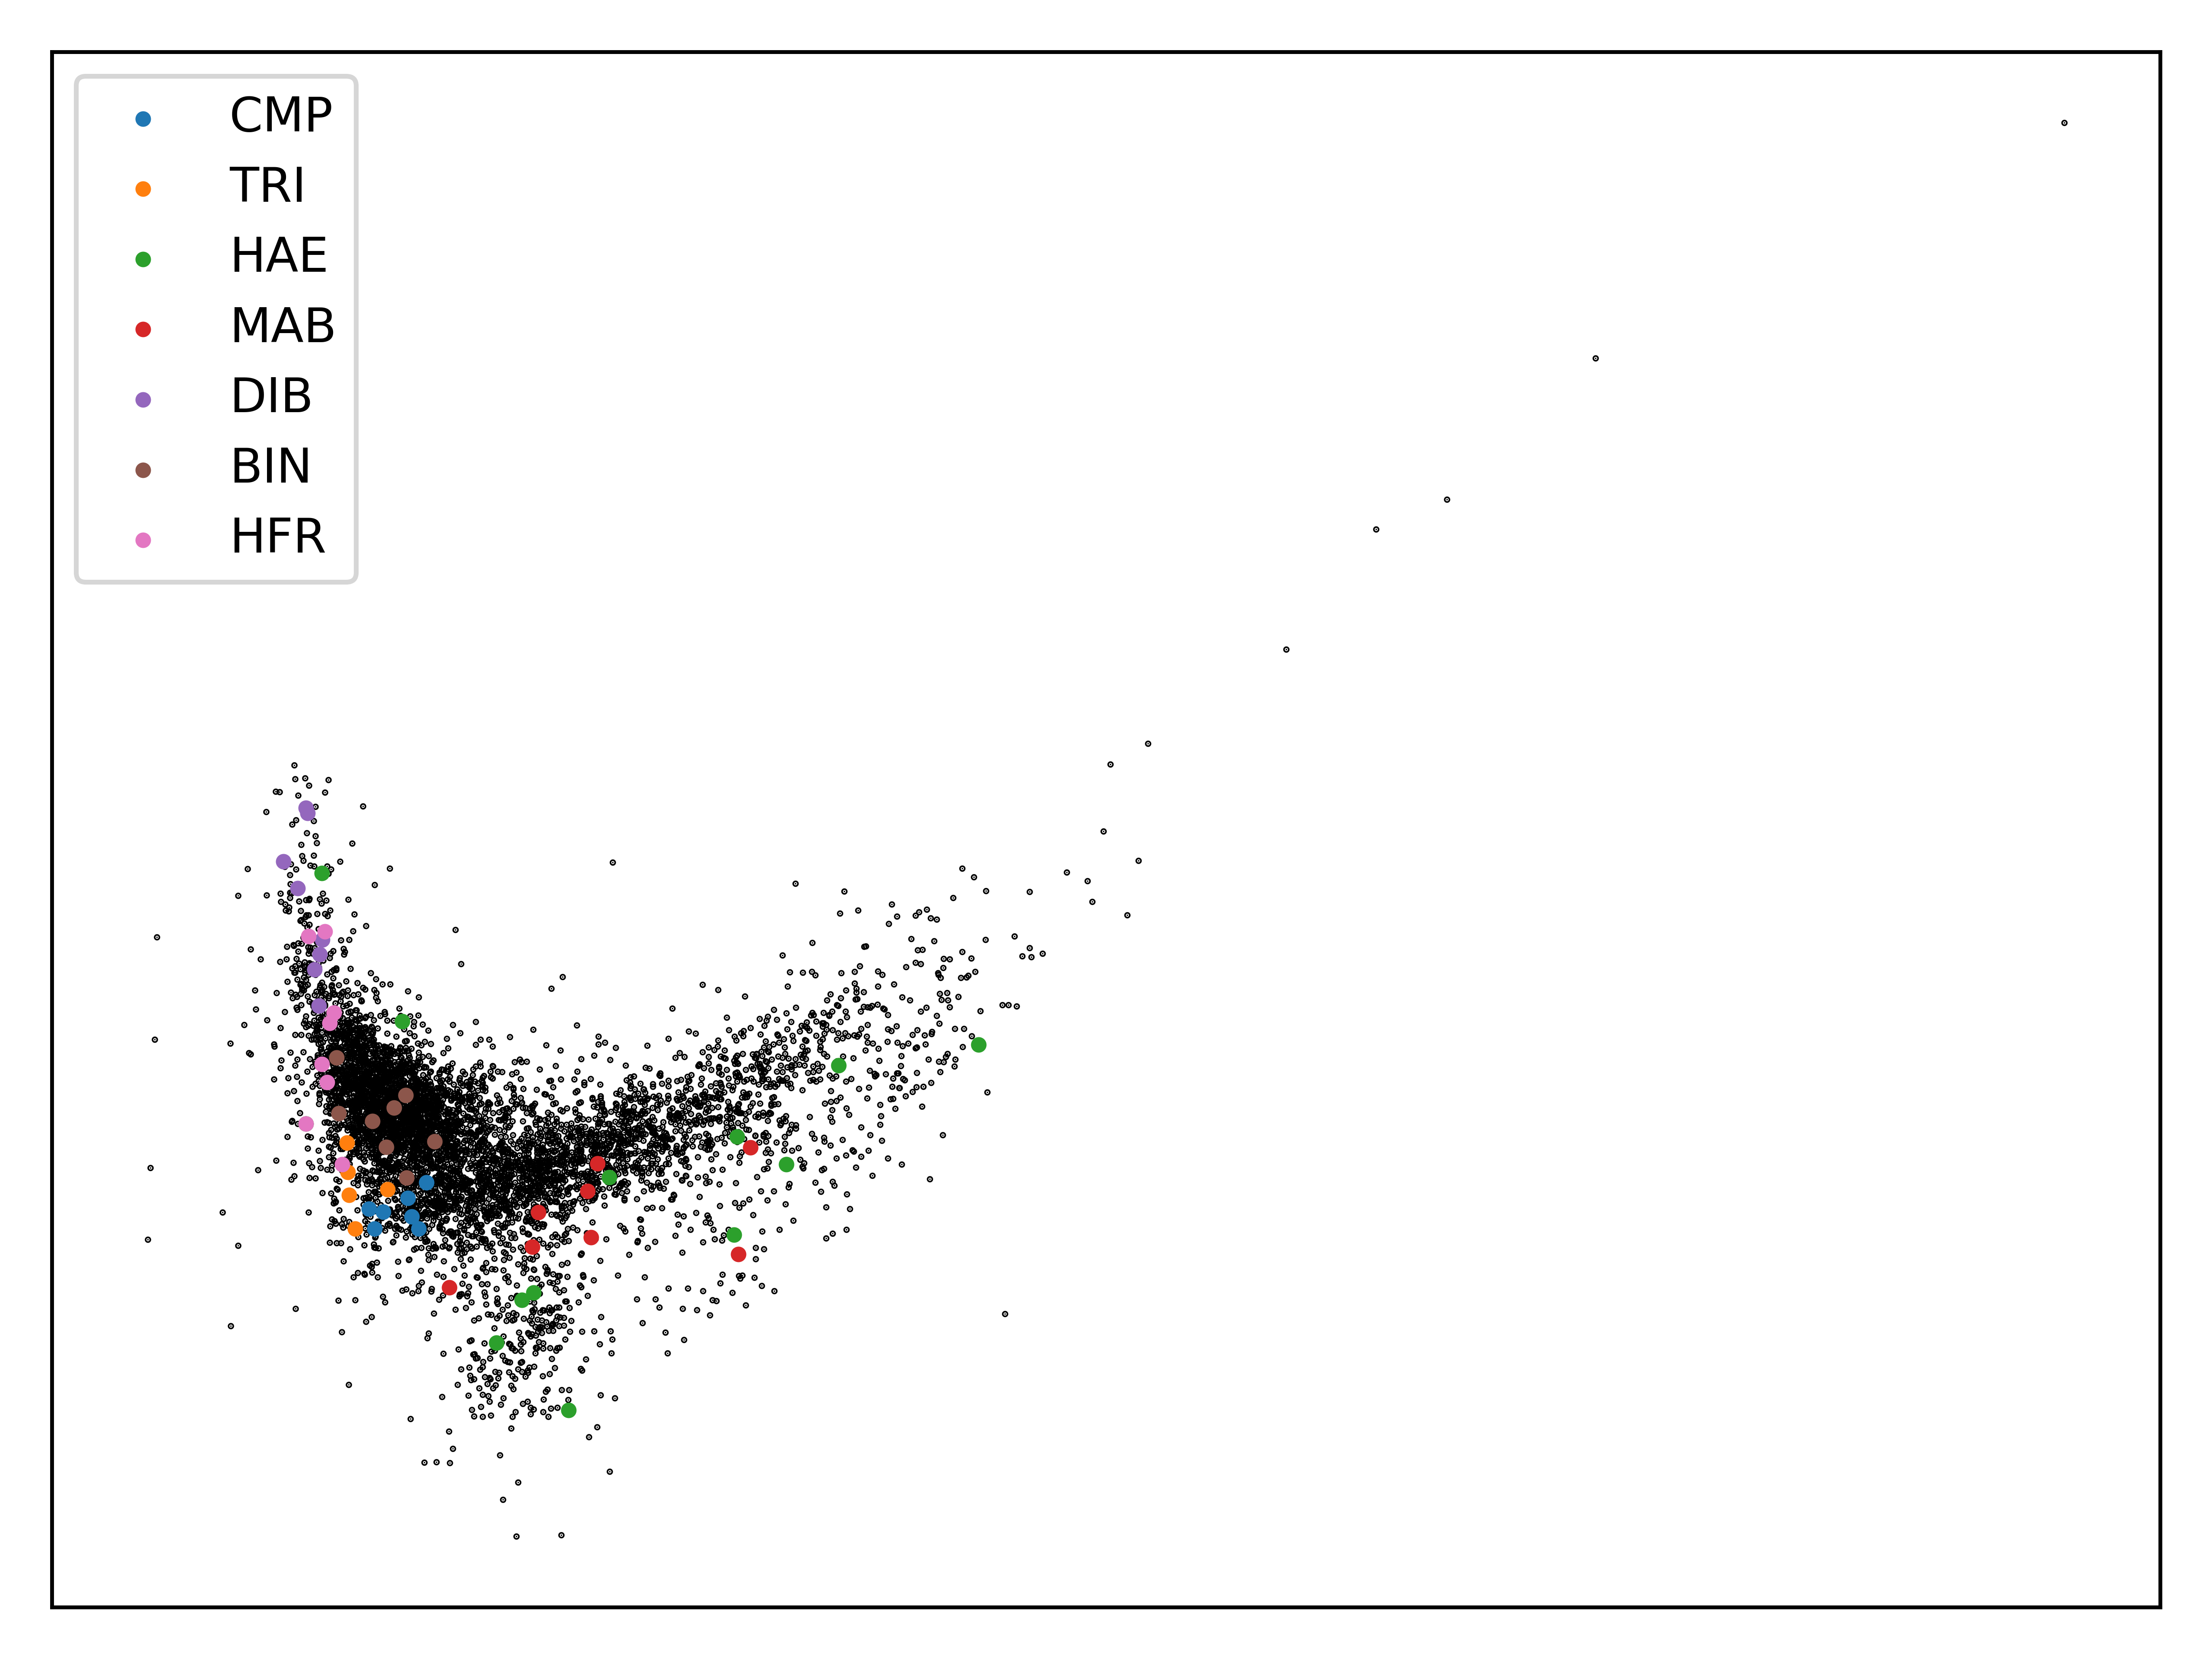
\includegraphics[width=\linewidth]{plots/PCA2D.png}
\end{subfigure}
\begin{subfigure}{.48\textwidth}
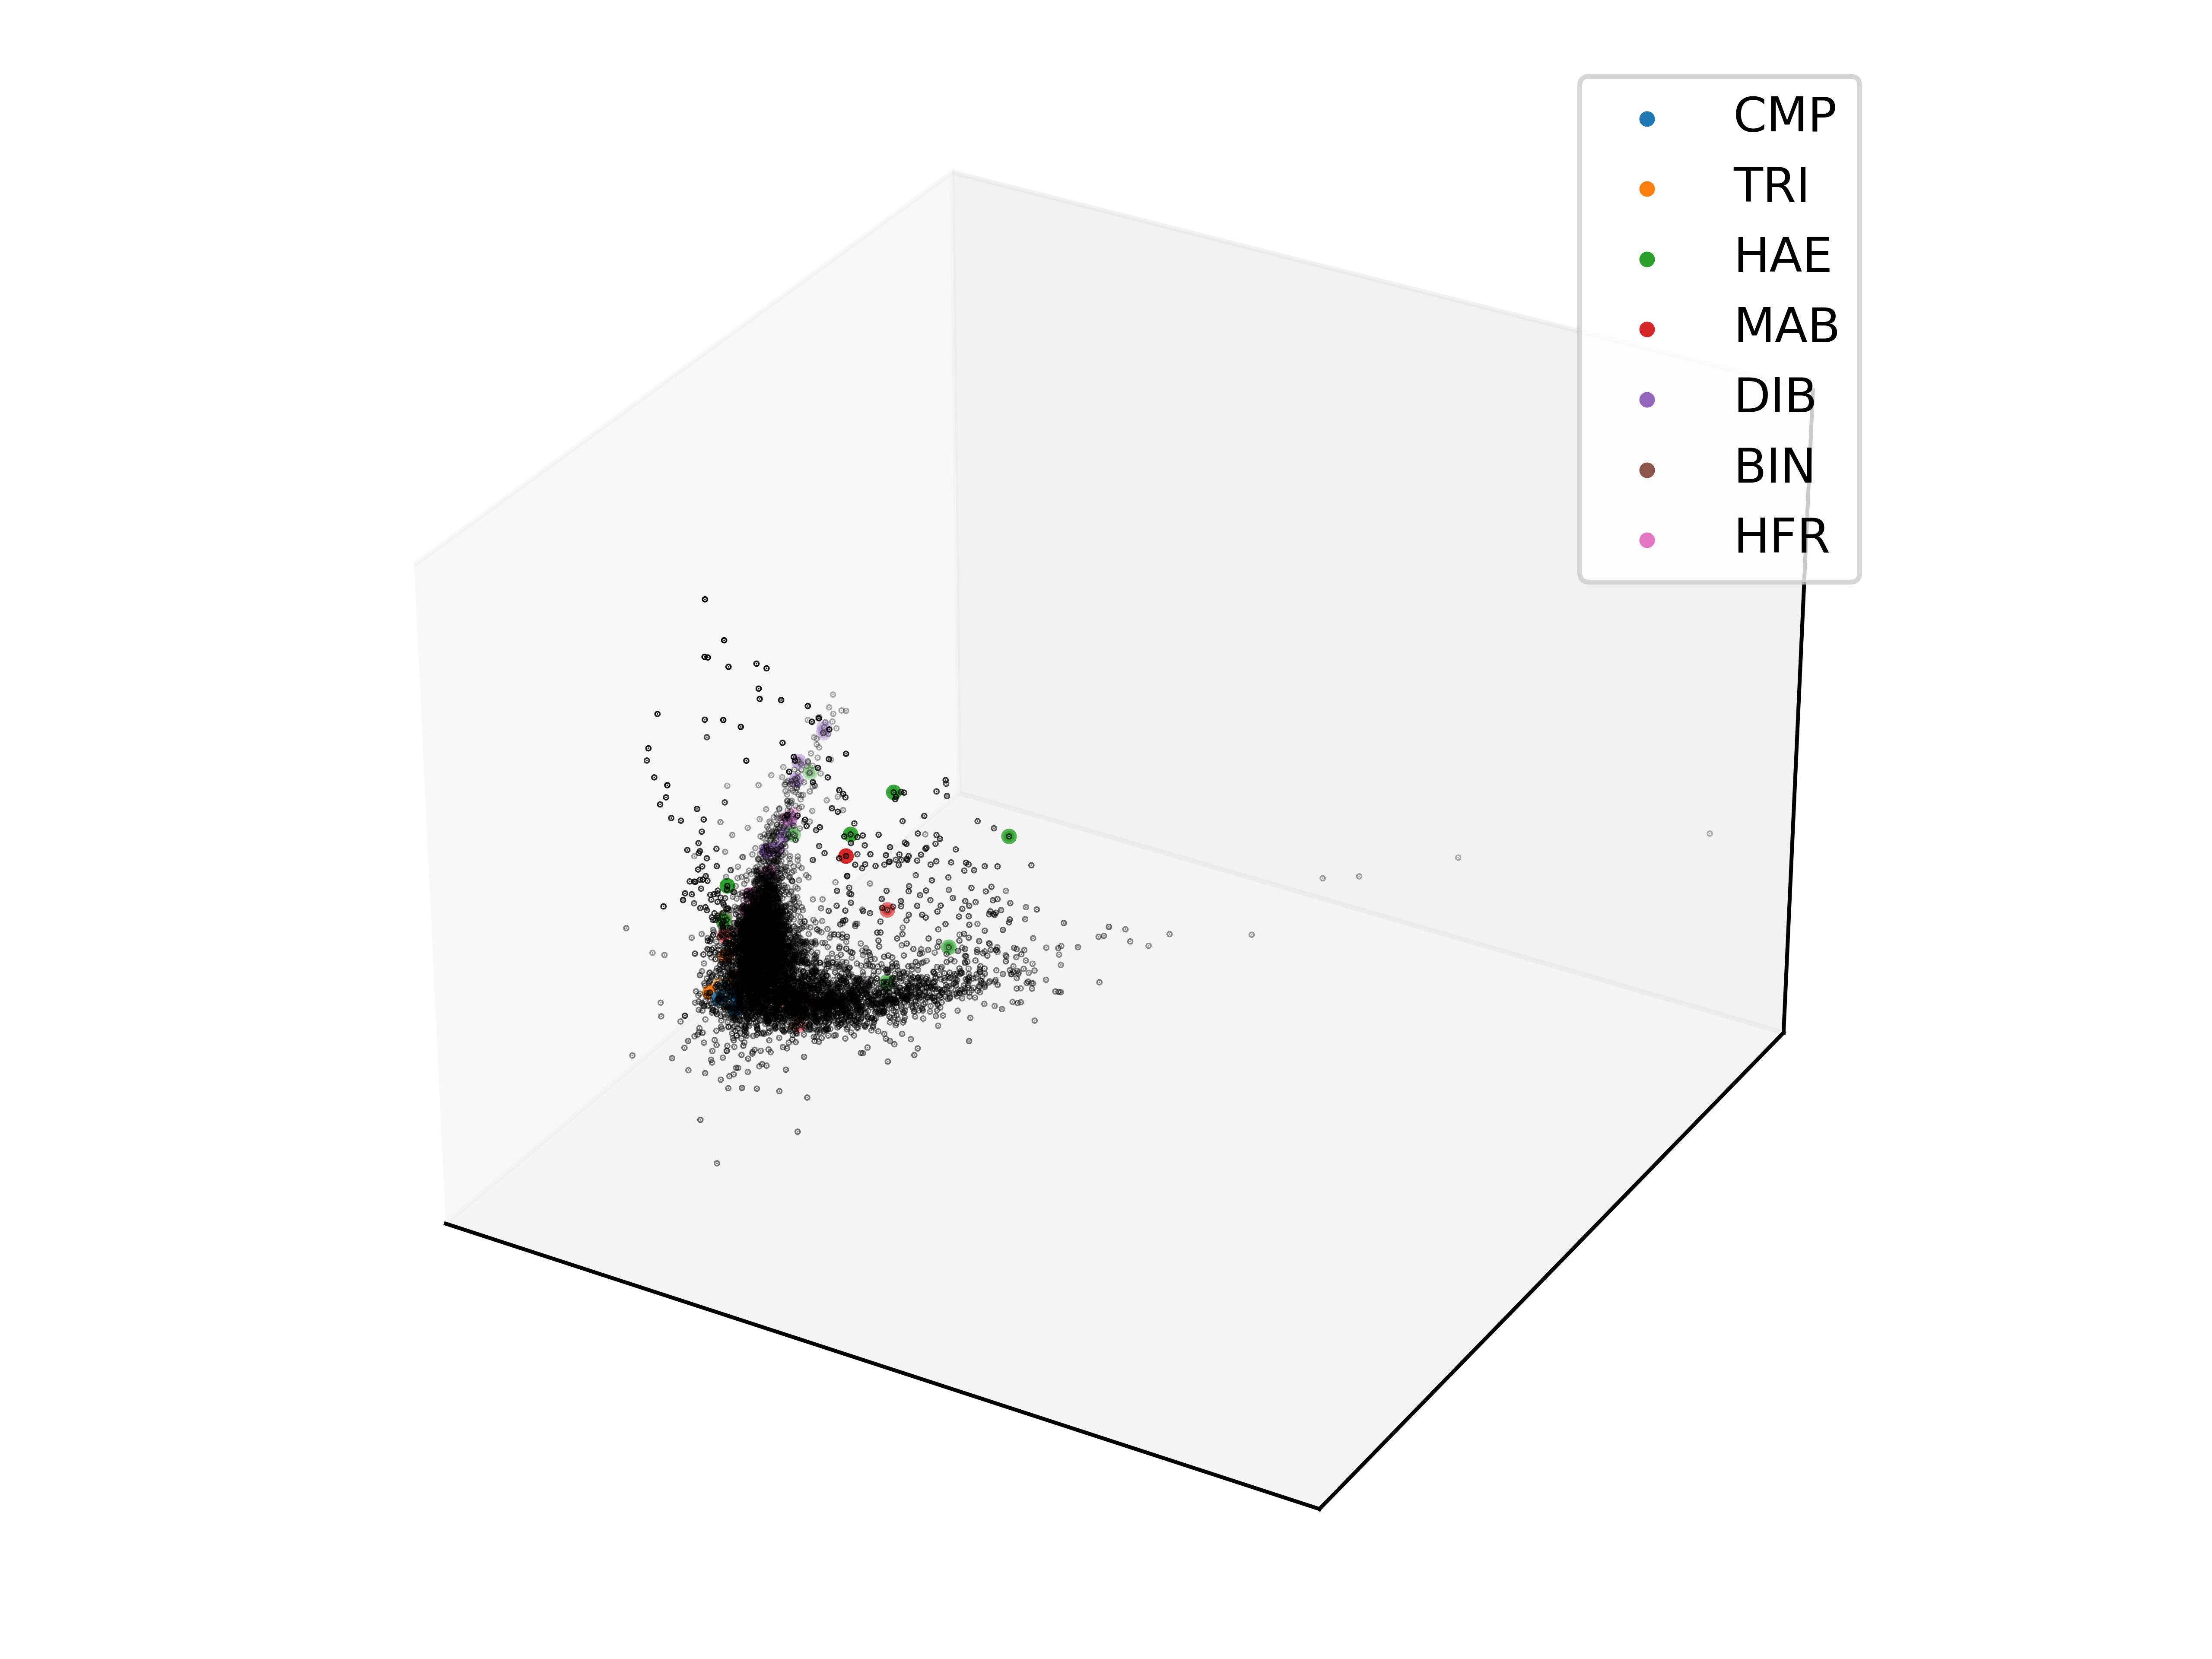
\includegraphics[width=\linewidth]{plots/PCA3D.png}
\end{subfigure}
\caption{PCA projection of the data to 2 and 3 dimensions}
\label{fig:PCA2D}
\end{figure}
There are also clear outliers in the data that should perhaps be removed. For now, we keep them and see if we can make sense of them.
Higher dimensional reductions are still possible but very undesirable (We want to still be able to visually see how well seperated the different labels are before proceeding to the next step). Out of curiosity, let us try some. We could visualize 4D in the same manner as before (4th dimension being color), but this would make it difficult to show where the annotated data lies, so let's opt for a corner plot, seen on Figure \ref{fig:corner}, where we project to 6 dimensions and plot the components pairwise against each other. Again, we see that the HAE data is all over the place and overlapping with others so it does not seem that the PCA approach will lead us anywhere.

\begin{figure}[H]
\centering
\begin{subfigure}{.7\textwidth}
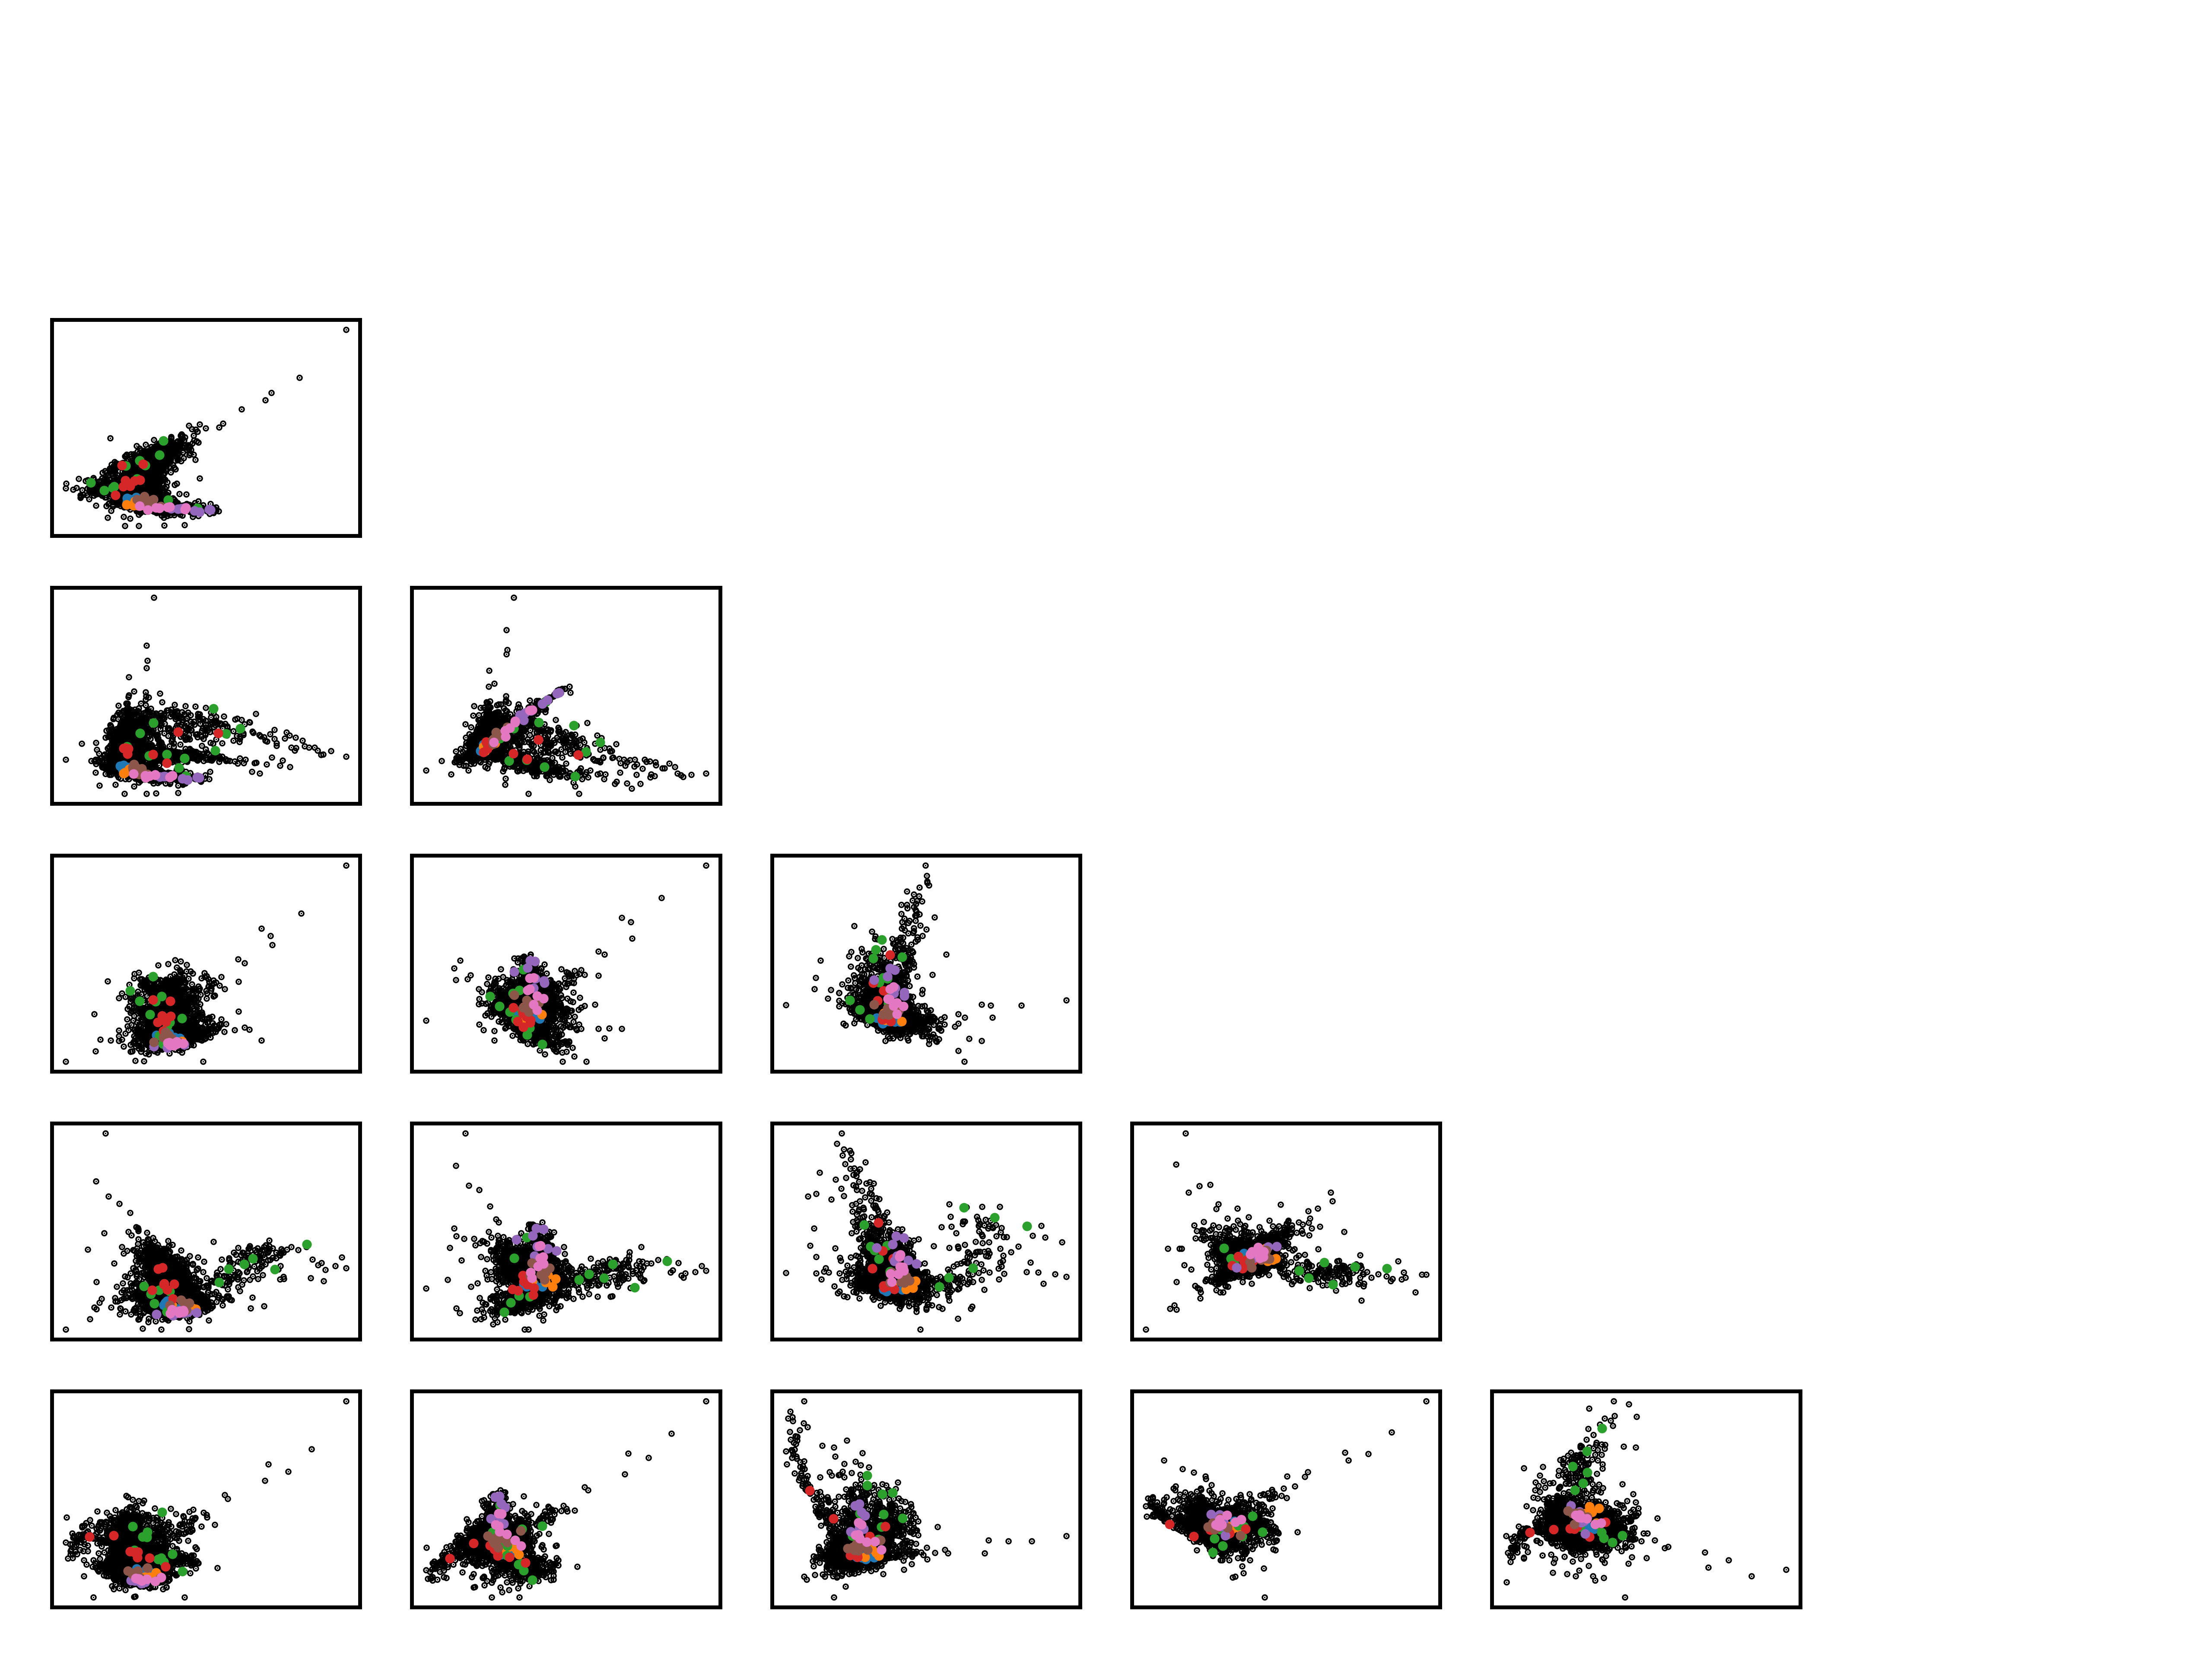
\includegraphics[width=\linewidth]{plots/PCA6D.png}
\end{subfigure}
\caption{PCA projection of the data to 6 dimensions shown as a corner plot.}
\label{fig:corner}
\end{figure}

Likely the problem is that the transformation that we have used so far is linear. We can introduce nonlinearity with kernel trick. The results for some kernels can be seen on Figure \ref{fig:kernelPCA}.
The linear kernel is equivalent to what we have seen before and just here as a reference. Poly kernel did a very bad job and is not even shown. For others, the shape parameter gamma has been left at a default value of around $~1/2084$ and not fine-tuned further. The results are alot better, with RBF kernels almost able to visually seperate the labelled spectra, although there are still some rogue points. I will move on to other techniques but return to this one and fine-tune the parameters if the others are not doing much better. 

\begin{figure}[H]
\centering
\begin{subfigure}{.7\textwidth}
\includegraphics[width=\linewidth]{plots/KernelPCA.png}
\end{subfigure}
\caption{PCA projection of the data to 2 dimensions with some different choices of kernels.}
\label{fig:kernelPCA}
\end{figure}

Let us move to a different form of dimensionality reduction all-together. We no longer project but instead employ manifold learning and try to learn an embedded manifold that the data may lay on.
For this, I will use the Locally Linear Embedding method, which tries to construct a manifold that in a sense maintains the neighbourhoods in the original data. The results can be seen on Figure \ref{fig:LLE}, where it doesn't seem that the method works any better than kernel PCA. The legend has been omitted for clarity, but the colours have retained their meaning from the previous plots.

\begin{figure}[H]
\centering
\begin{subfigure}{.7\textwidth}
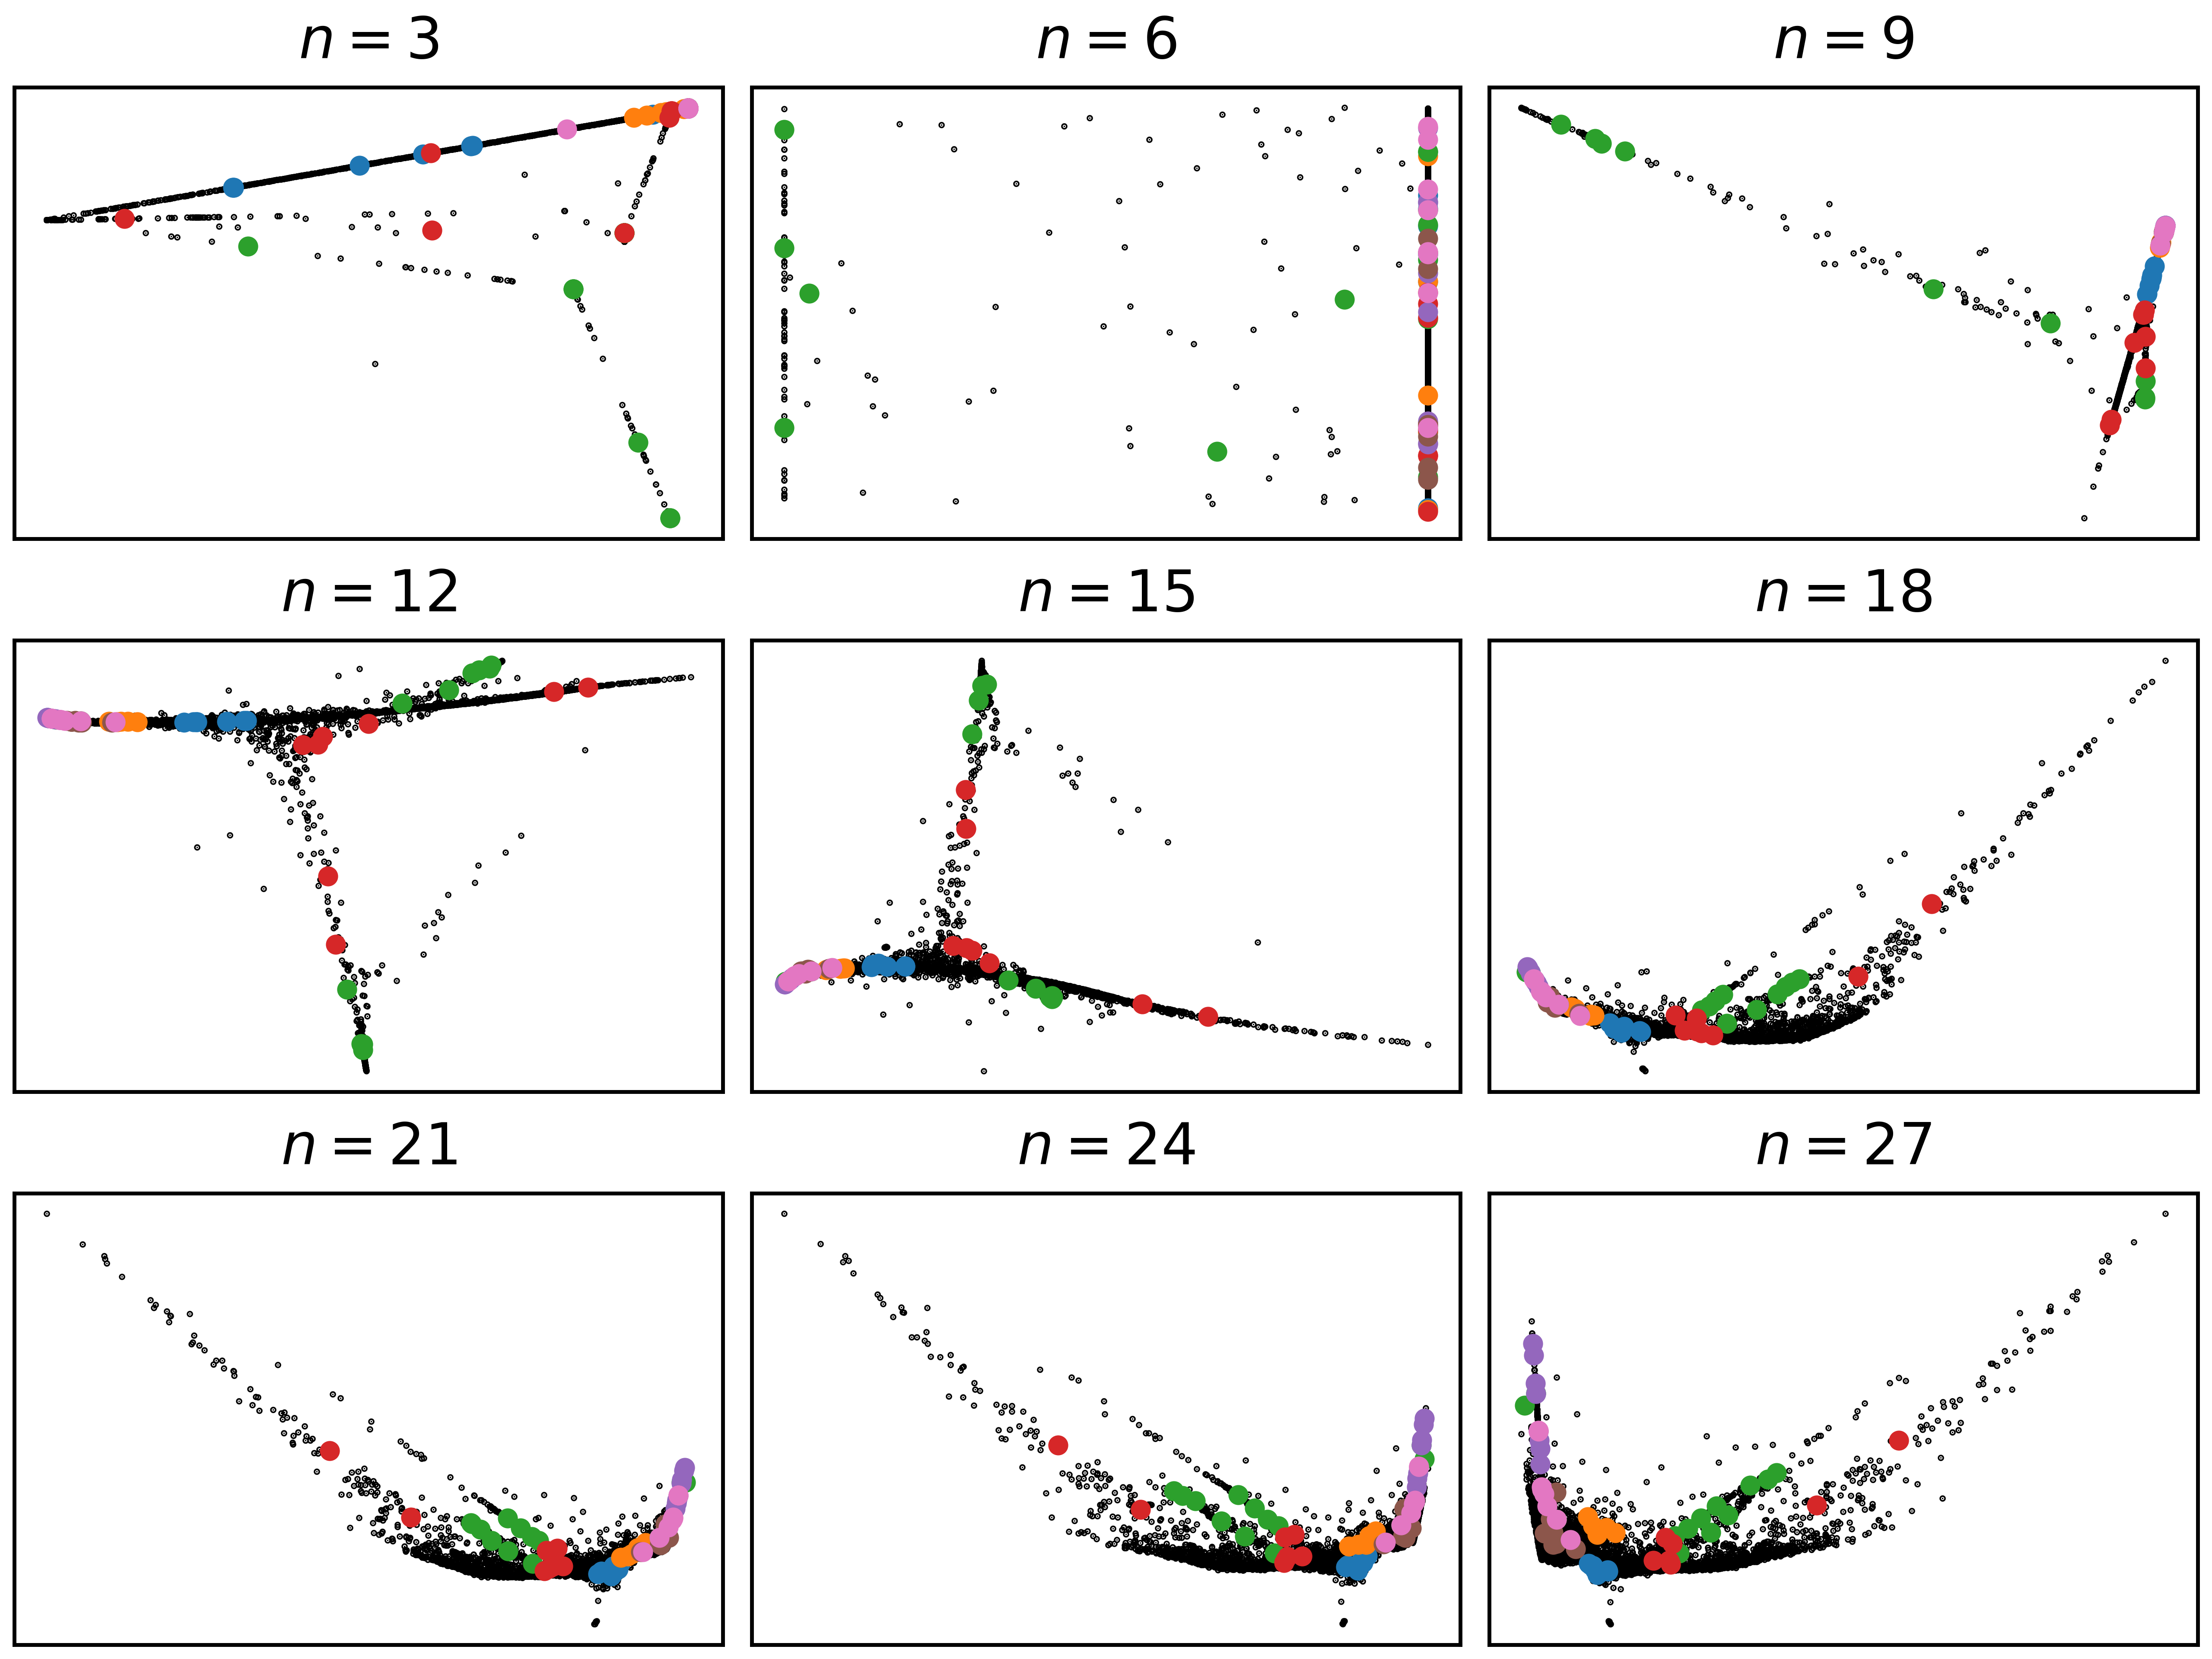
\includegraphics[width=\linewidth]{plots/LLE.png}
\end{subfigure}
\caption{LLE dimensionality reduction. The parameter $n$ is the size of the neighbourhood and a parameter of the method.}
\label{fig:LLE}
\end{figure}

As a last method we test one of the most famous dimensionality reduction methods (apart from PCA), the tSNE method. The results are seen on Figure \ref{fig:tsne}. The parameter of the method is perplexity, which is the power of the entropy of the distribution in the original data space. The values of the perplexity parameter have been chosen in the suggested range of $[5,50]$.
As usual, we use the more efficient Barnes-Hut tSNE approximation. This is still quite inefficient so we first PCA project to a dimensionality of 100 and only then follow up with a tSNE. We rerun the tSNE algorithm 10 times and pick the one with lowest KL divergence value.

\begin{figure}[H]
\centering
\begin{subfigure}{.7\textwidth}
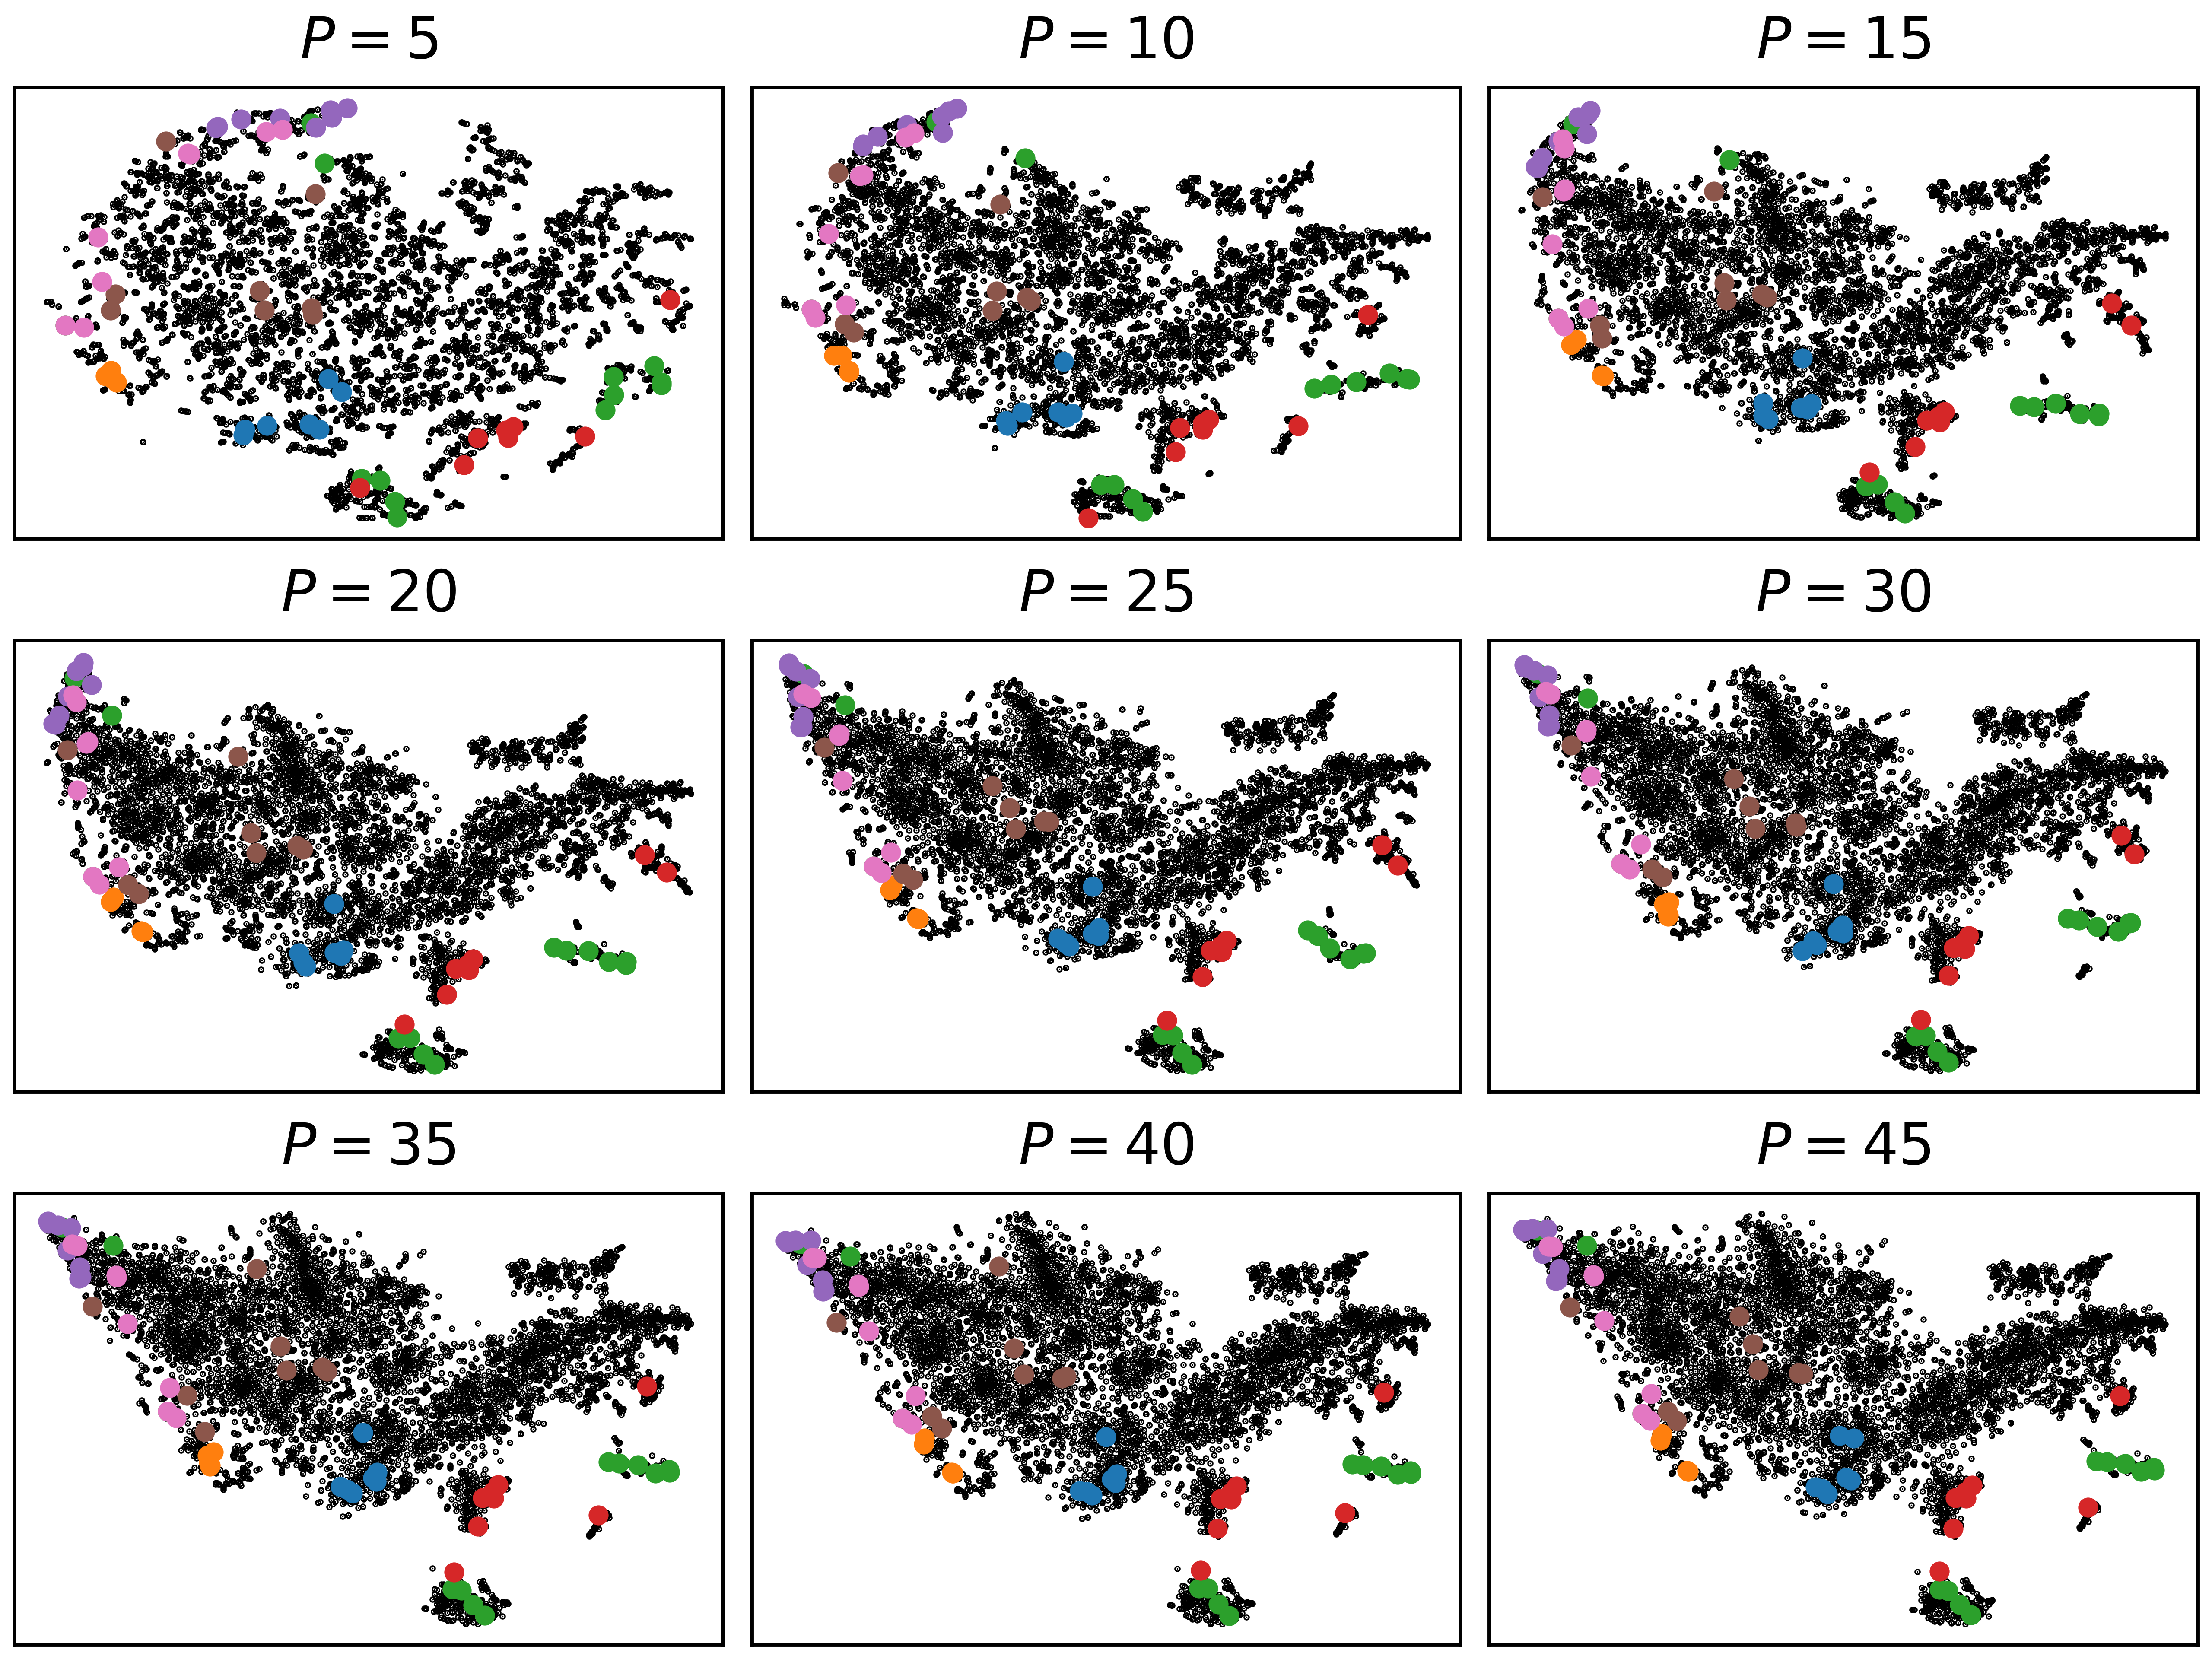
\includegraphics[width=\linewidth]{plots/tsne.png}
\end{subfigure}
\caption{tSNE reductions for different values of perplexity ($P$).}
\label{fig:tsne}
\end{figure}

We were not able to find a perfect low-dimensional representation of the data, that would clearly seperate the labeled data. It might be valuable to invest more time in fine tuning our approaches, but let's instead get at least some sort of answer and classify the best we can with what we have available. Visually, it seems P=15 tSNE seems to have seperated the data the best. 

\section*{Classification}
In this section, we will classify the reduced spectra, obtained from $P=15$ tSNE.
For the classifier, let's first try logistic regression. That is, we simply start with a usual regression and then apply the sigmoid function (changing the range to $(0,1)$) and train it on the data. By default the regression step is linear with an L2 regularizer.
The result can be seen on Figure \ref{fig:logistic}.
We can see that majority of the points are classified as the problematic HAE type, even though visually it seems that the bottom right should perhaps be MAB instead.

\begin{figure}[H]
\centering
\begin{subfigure}{.7\textwidth}
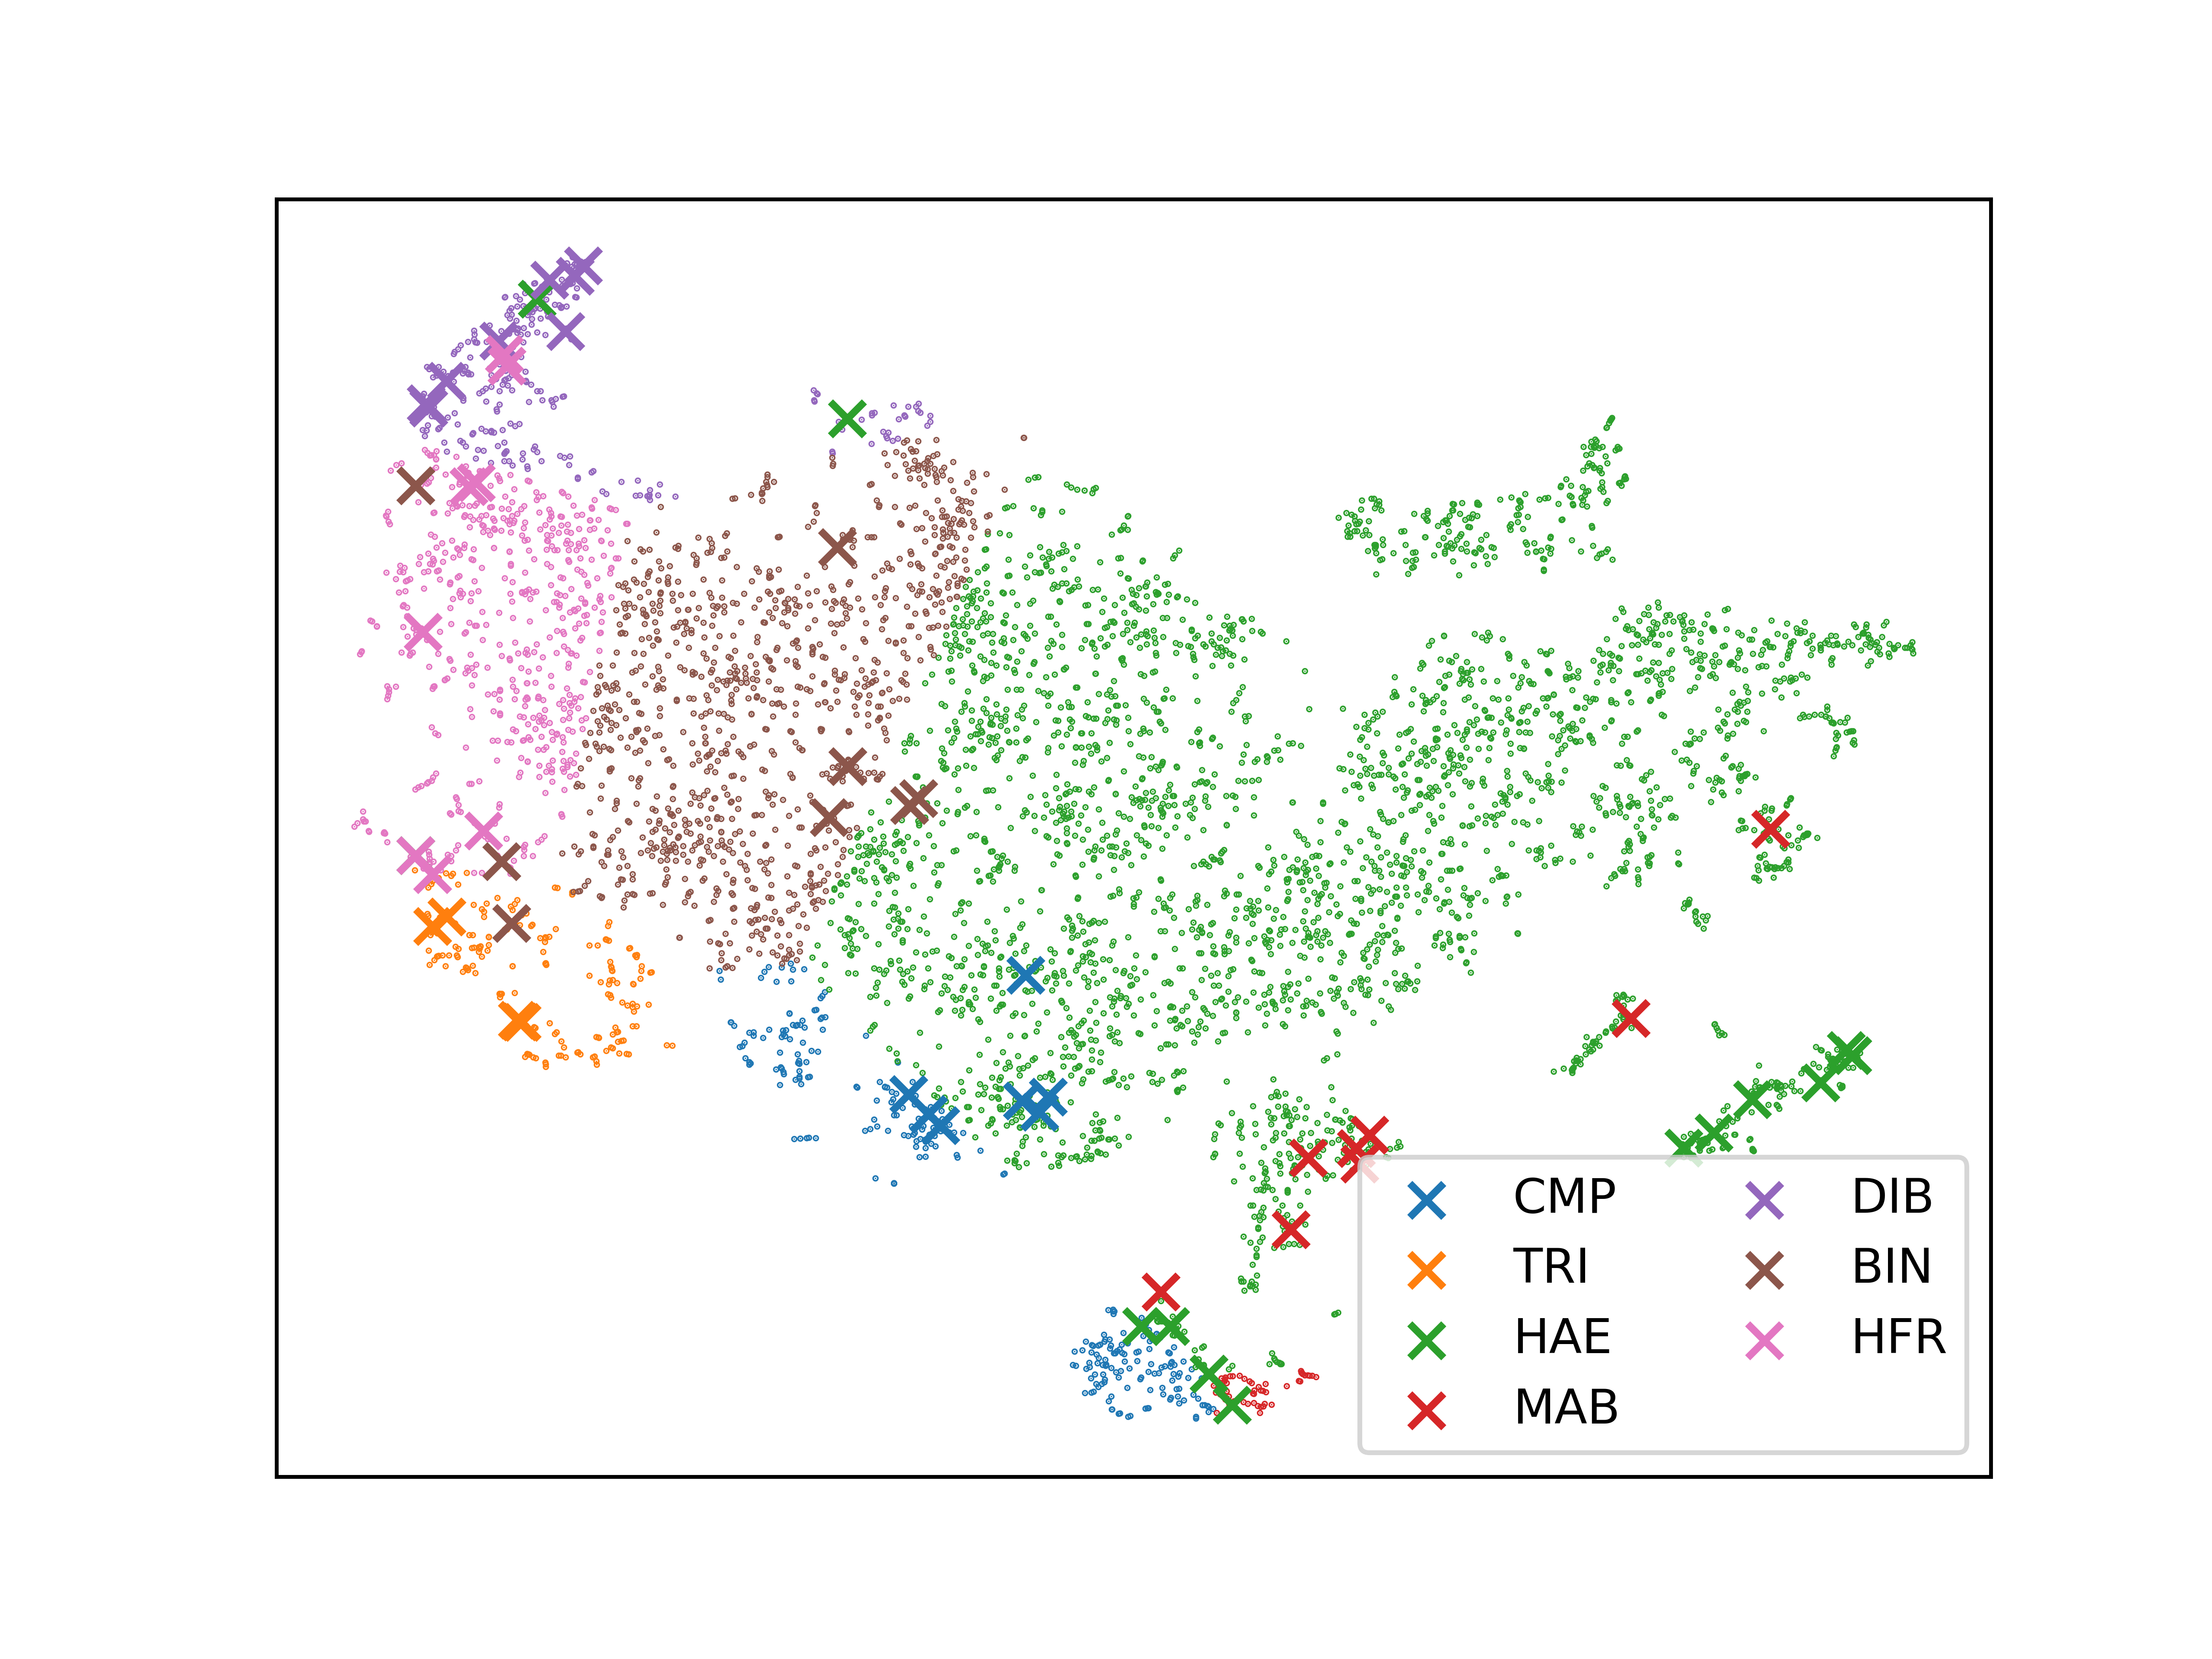
\includegraphics[width=\linewidth]{plots/logistic1.png}
\end{subfigure}
\caption{Classification with logistic regression. The crosses represent labelled data, while the dots the classified ones.}
\label{fig:logistic}
\end{figure}

Let us try to improve that classification by first using more features, expanding to include up to 3rd power of the data (again feature expension in the regression algorithm). The results can be seen on Figure \ref{fig:logistic3}. This looks alot better.

\begin{figure}[H]
\centering
\begin{subfigure}{.7\textwidth}
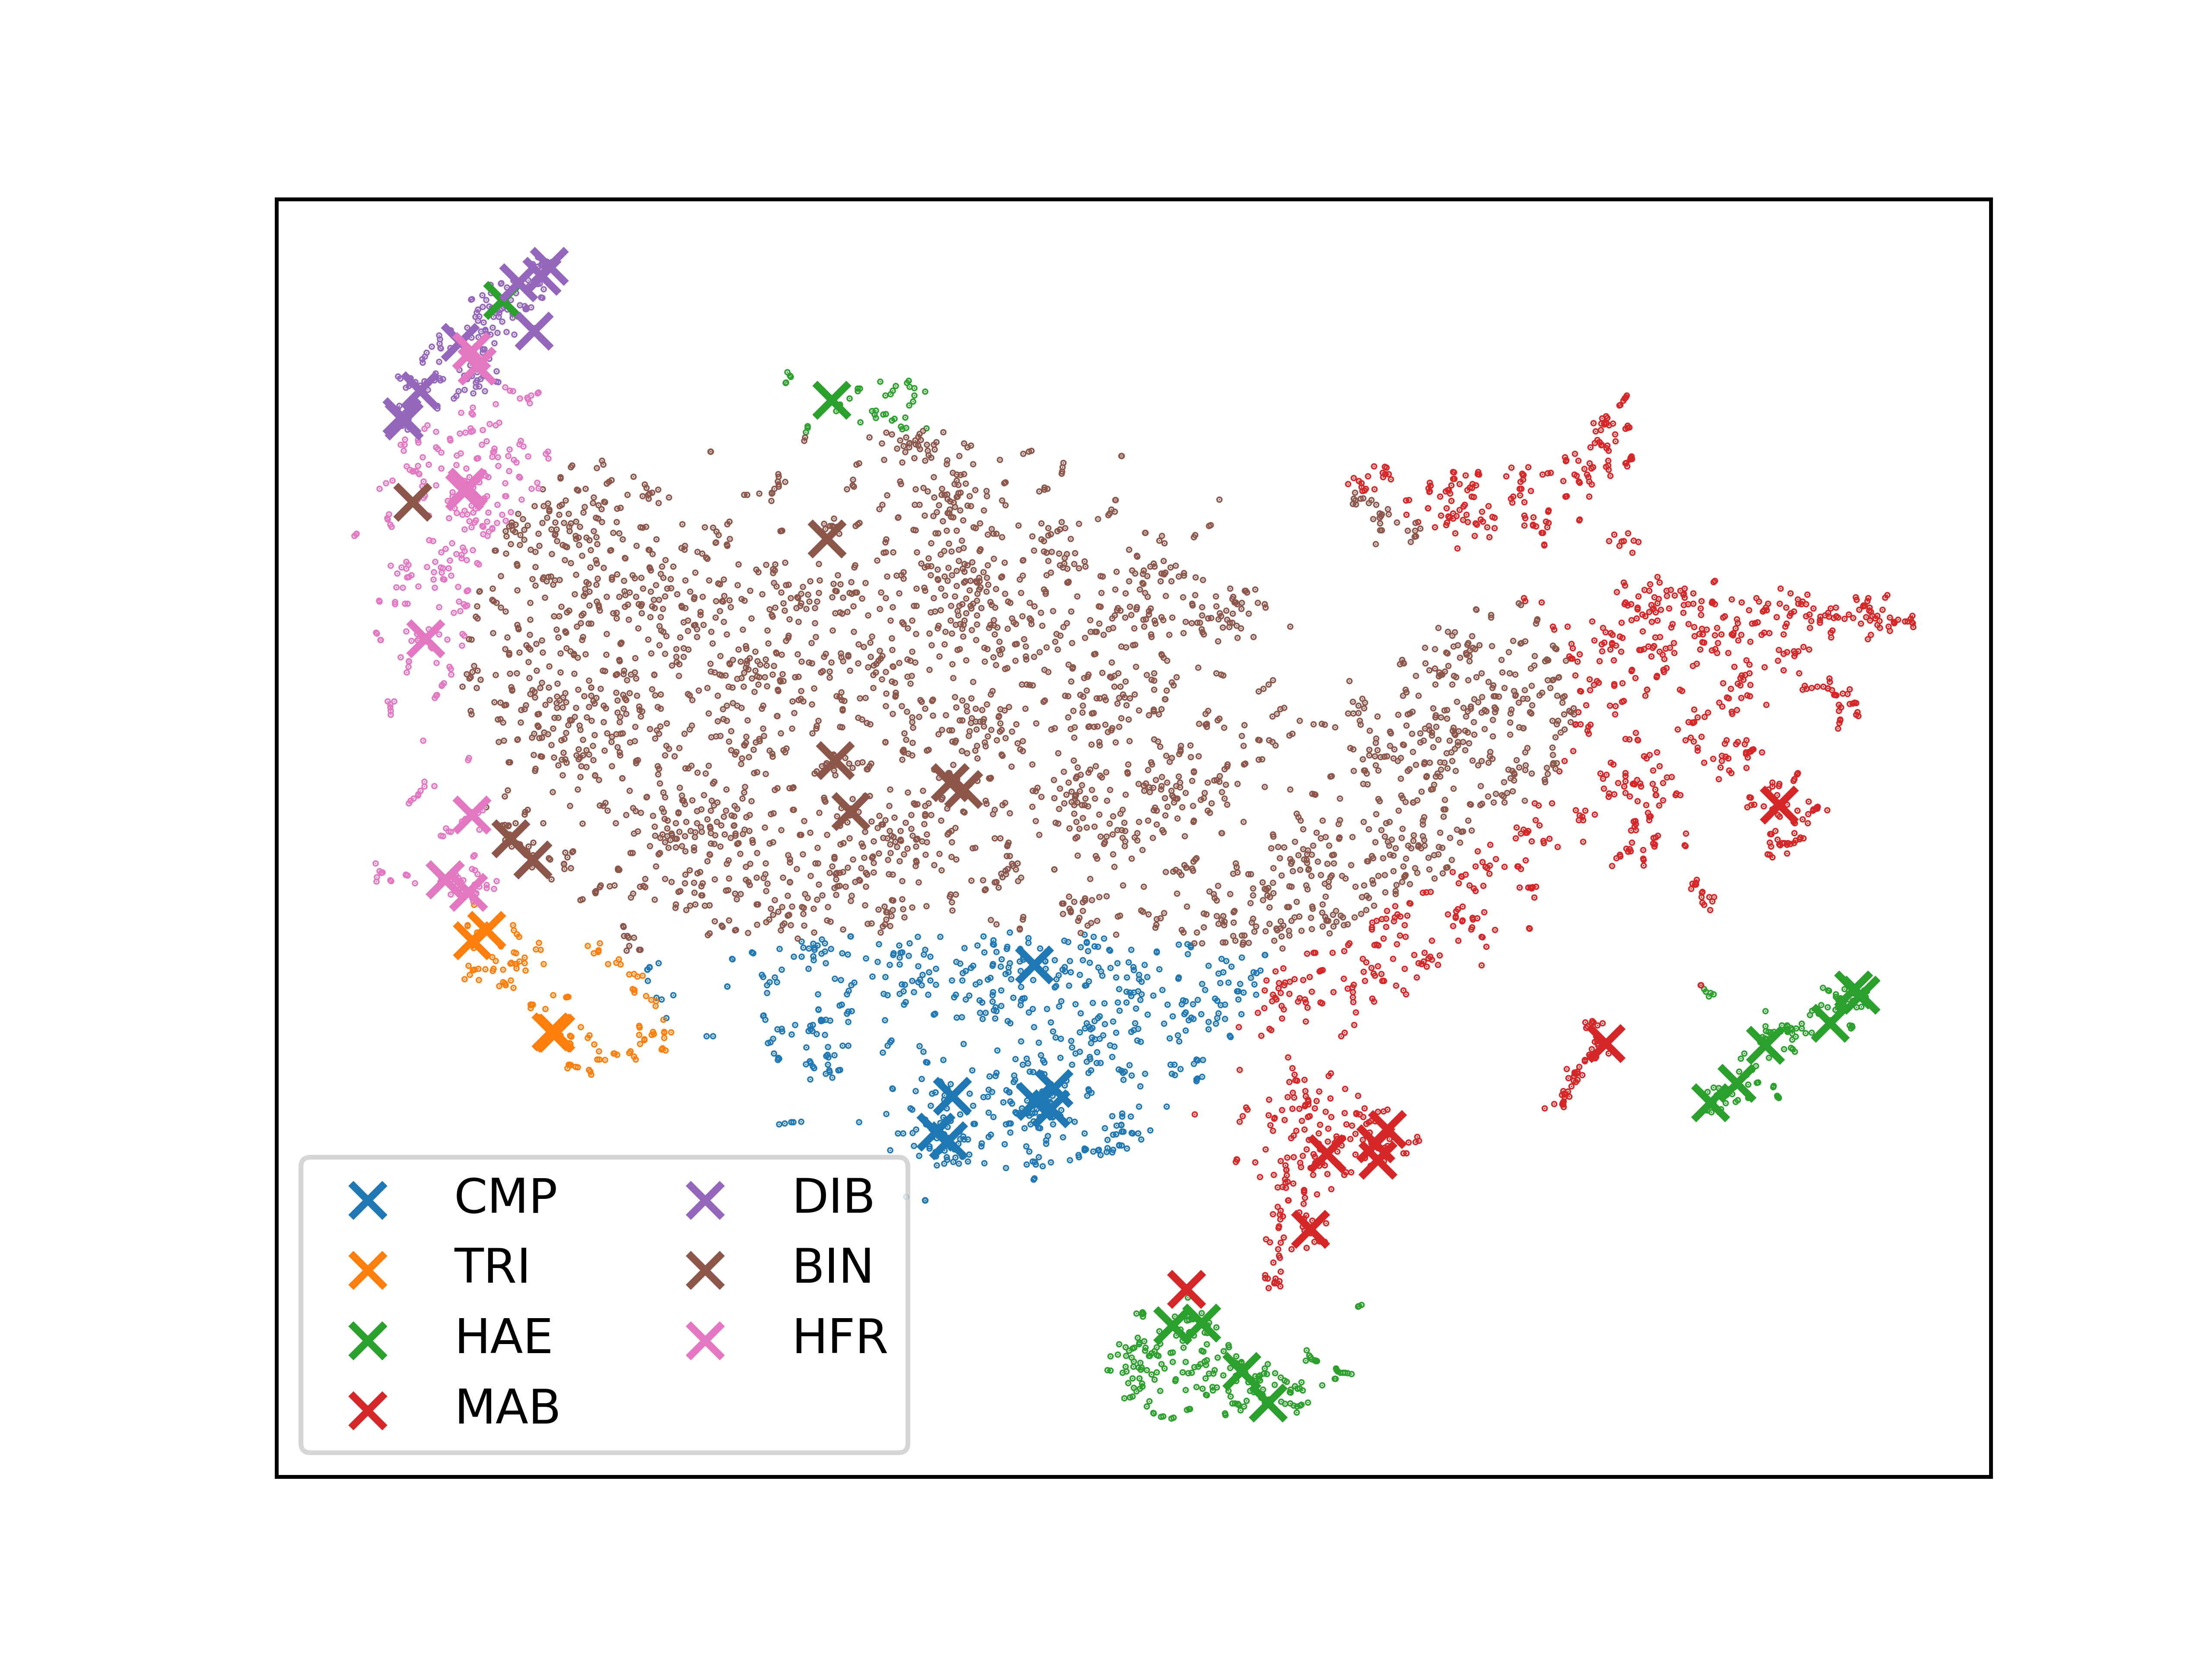
\includegraphics[width=\linewidth]{plots/logistic3.png}
\end{subfigure}
\caption{Classification with logistic regression (3rd degree polynomial interpolation). The crosses represent labelled data, while the dots the classified ones.}
\label{fig:logistic3}
\end{figure}

For an even further improvement, we can use LogisticRegressionCV, which performs a grid search on the optimal regularization parameter. Results are seen on Figure \ref{fig:logisticCV3}. The results look even better and perhaps a completely satisfactory result, but for education purposes we still pursue other means.

\begin{figure}[H]
\centering
\begin{subfigure}{.7\textwidth}
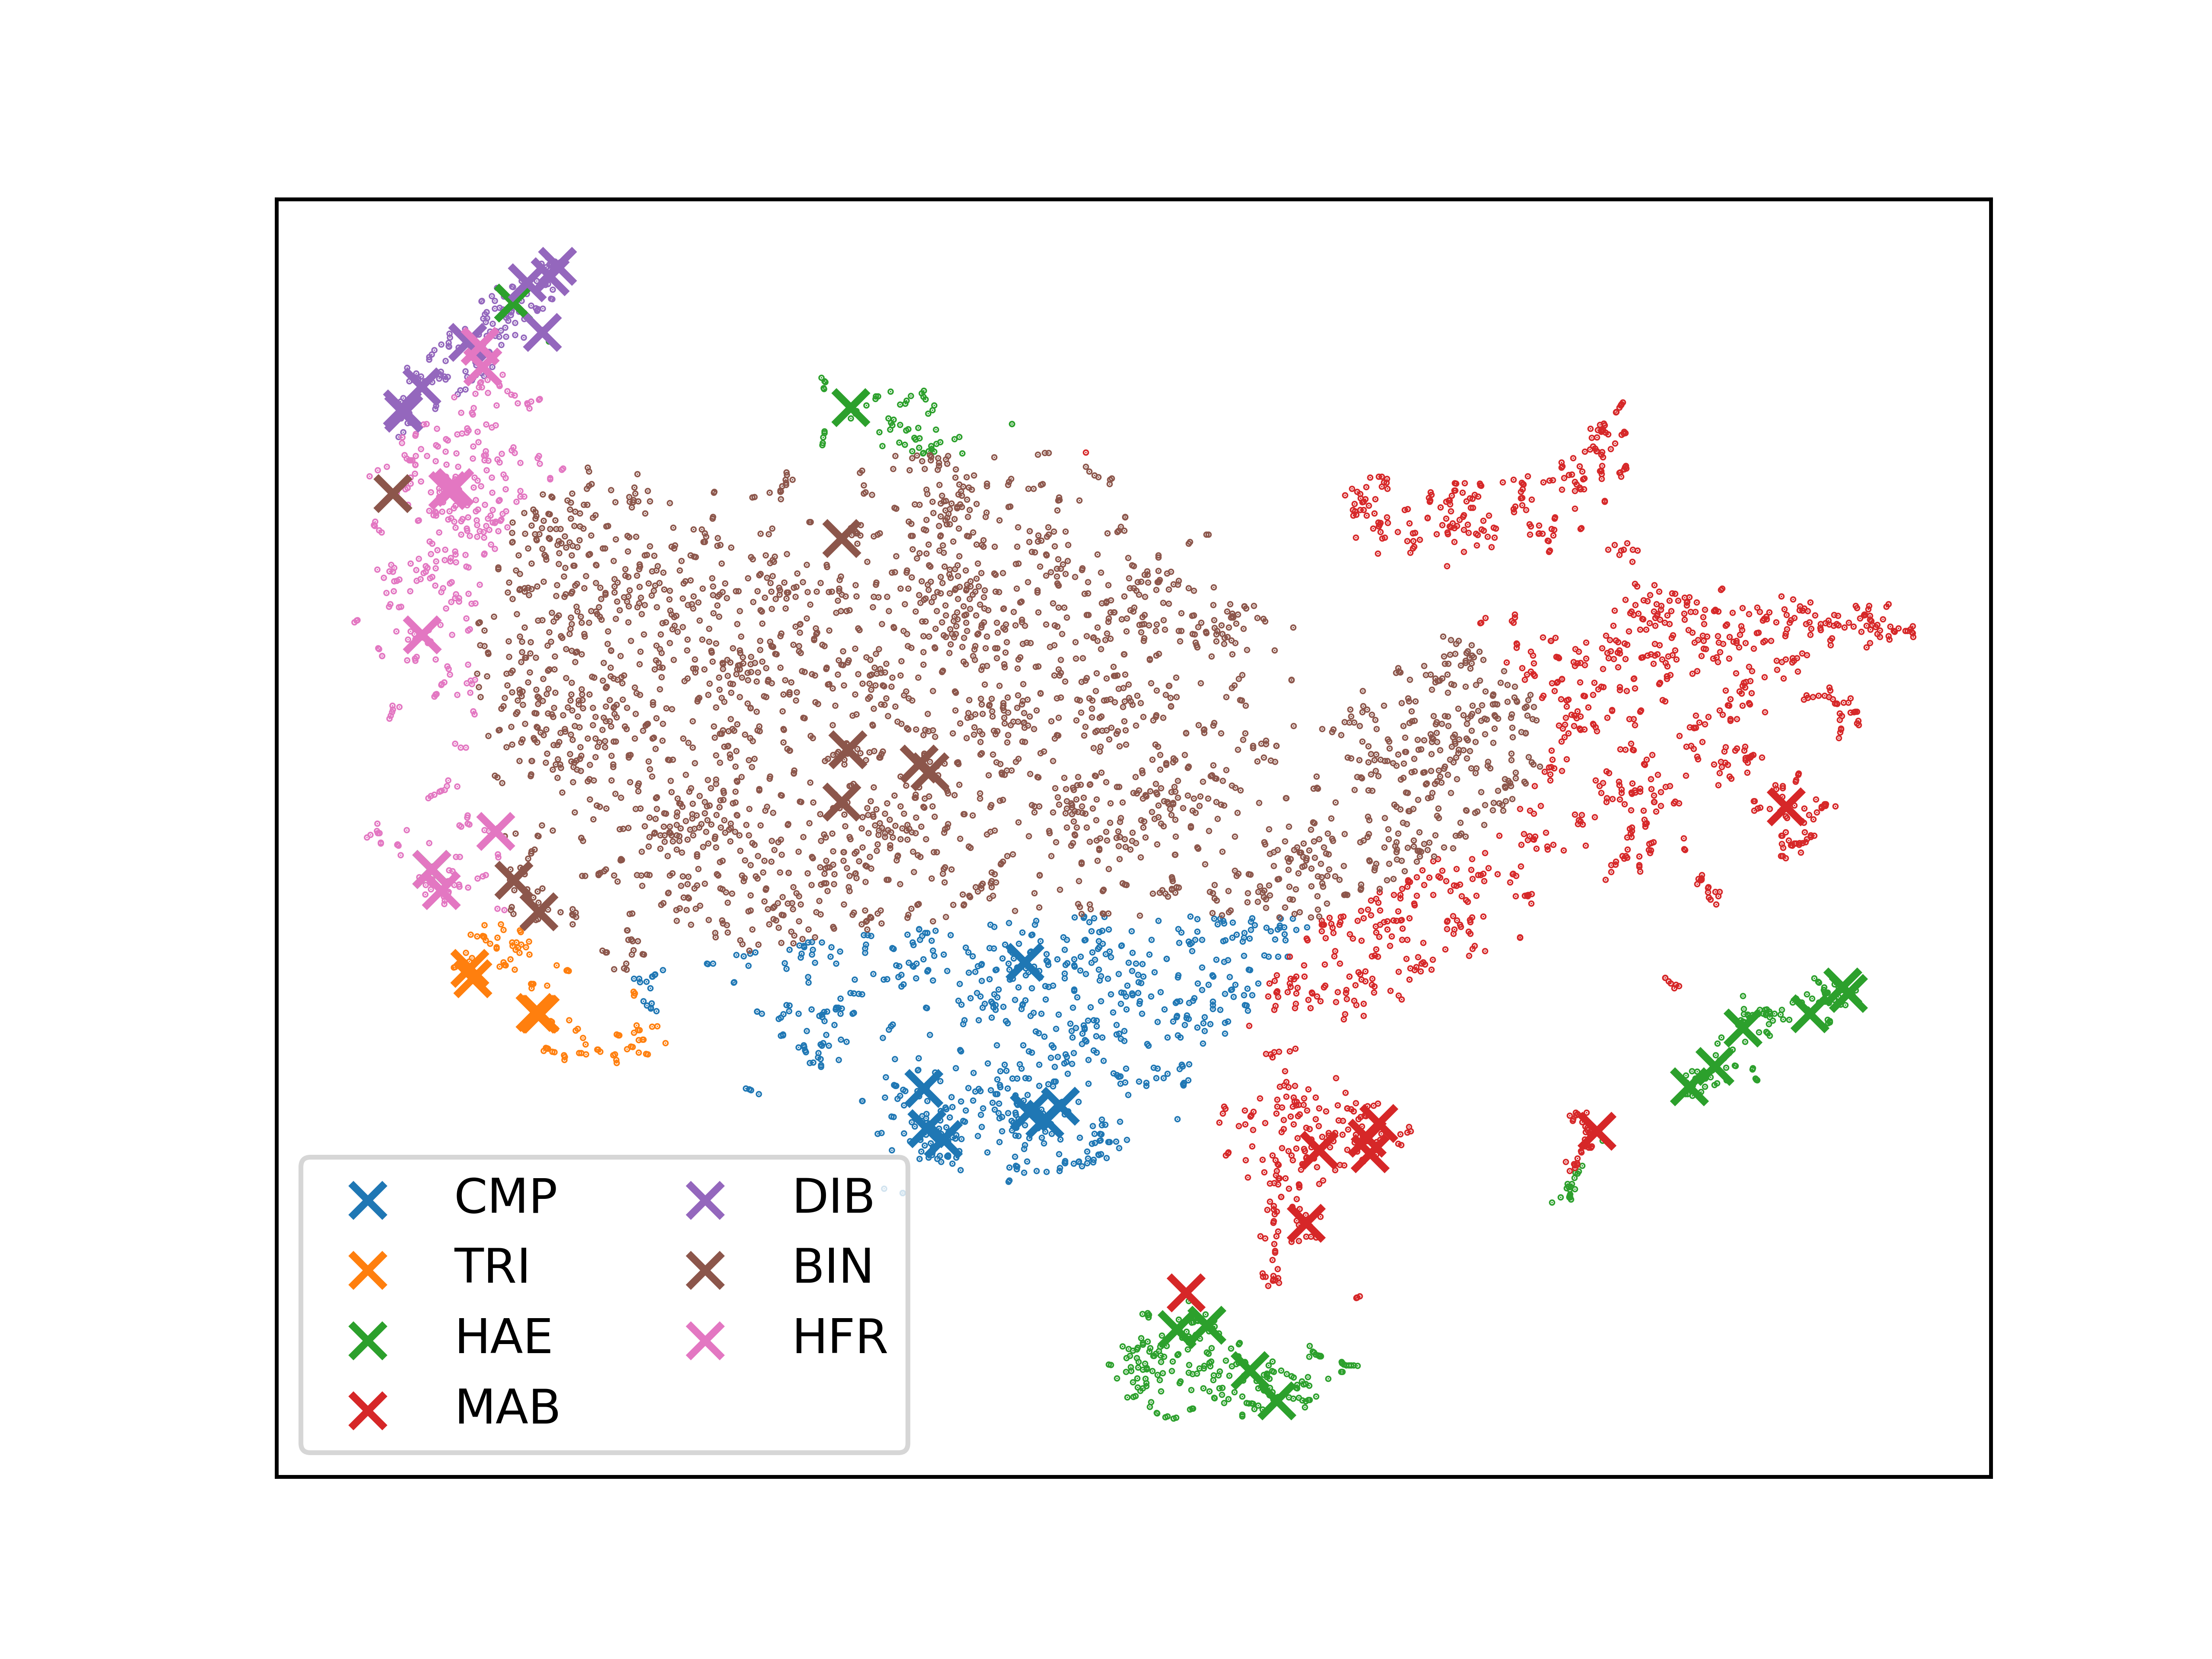
\includegraphics[width=\linewidth]{plots/logisticCV3.png}
\end{subfigure}
\caption{Classification with logistic regression (3rd degree polynomial interpolation) and CV. The crosses represent labelled data, while the dots the classified ones.}
\label{fig:logisticCV3}
\end{figure}

Next, instead of a sigmoid, we use a Heavyside step function, resulting in perceptron classification. The original regression is linear and without regularization and the optimal parameters are obtained using a Stochastic Gradient Descent. The results can be seen on Figure \ref{fig:perc}. It is quite similar to logistic regression, perhaps a bit better. When using the perceptron algorithm it is beneficial to use the usual DL techniques such as early stopping. Unfortunately, for our particular case this was not practical, because the number of labeled data is too small compared to the number of classes, which is probably why perceptron is not well suited for our case. Additionally, unlike logistic regression it only supports "one vs all" (classifying labels pairwise) classification, while logistic regression also supports the better suited multinomial method.

\begin{figure}[H]
\centering
\begin{subfigure}{.7\textwidth}
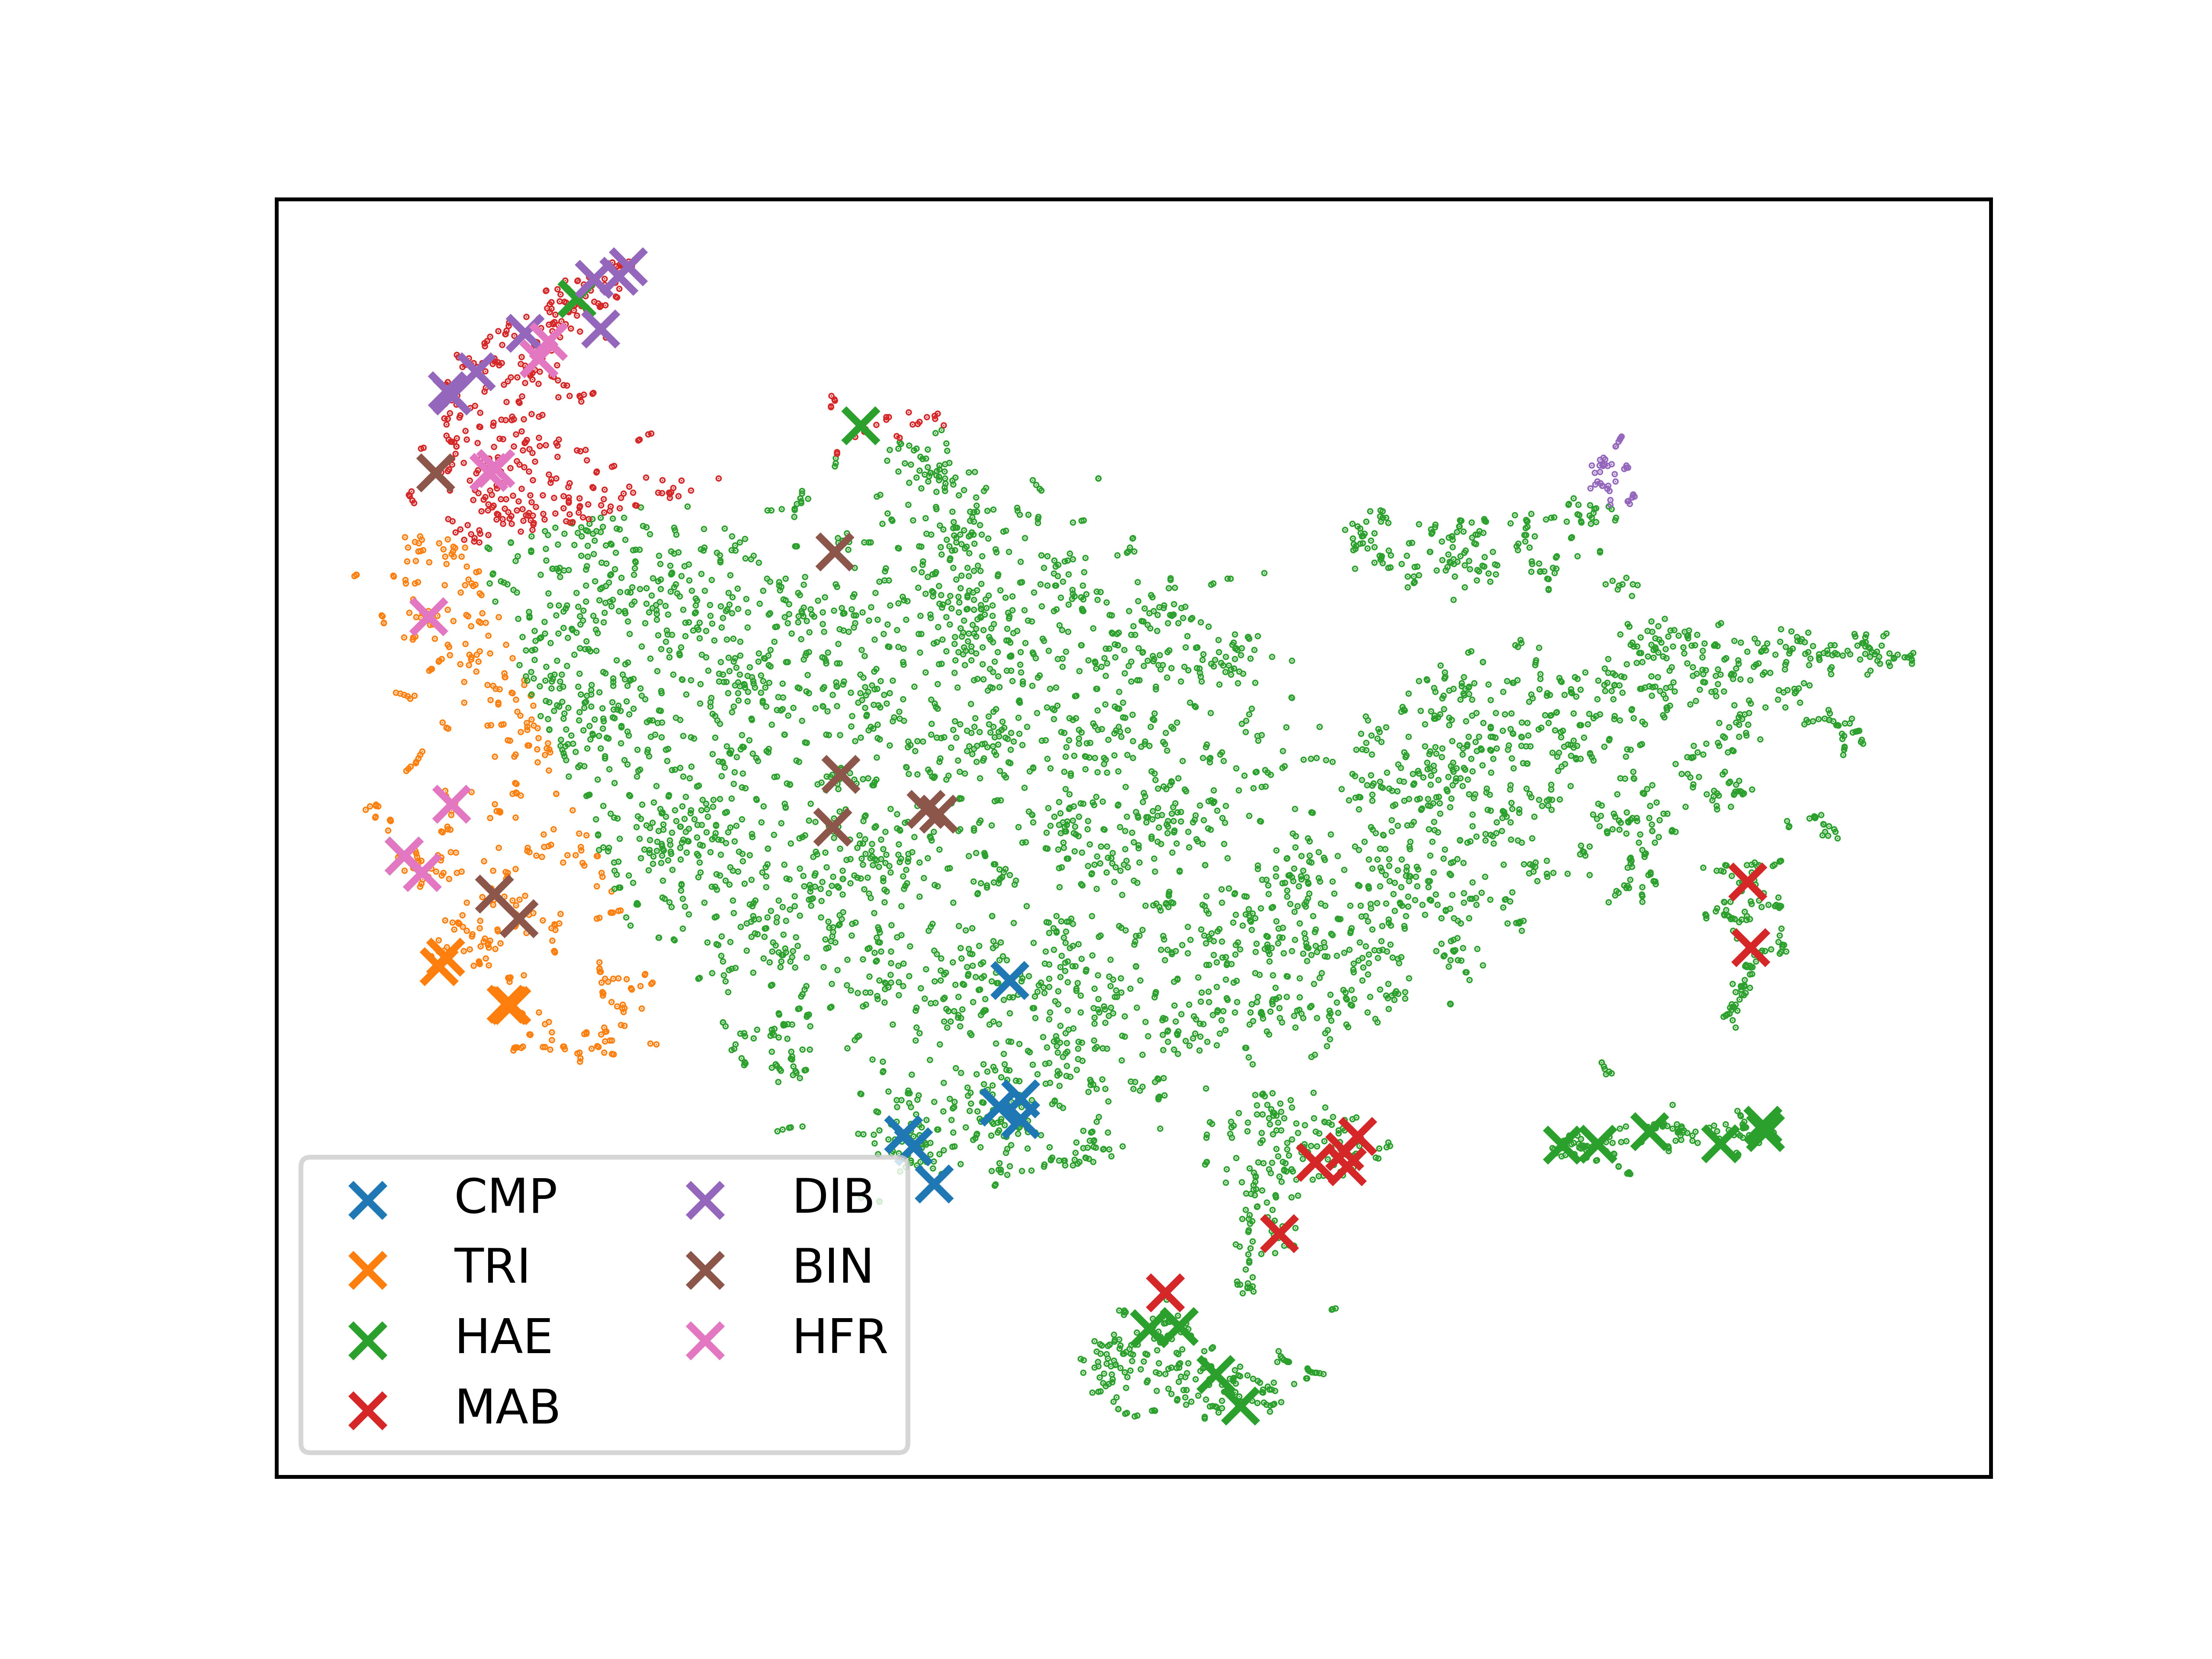
\includegraphics[width=\linewidth]{plots/perceptron.png}
\end{subfigure}
\caption{Classification with perceptron regression.}
\label{fig:perc}
\end{figure}

Let us reuse one more machinery from our regression project - Support Vector Machines, which we can use also for classification (SVC). This is shown on Figure \ref{fig:svc} for some different choices of kernels, allowing for more non-linear decision boundaries. The parameters have been left at their default value, that is the shape parameter $\gamma$ the inverse of the number of features multiplied by X.var(). The poly kernel degree is $3$. The RBF results seem pretty good, although some points (which may be just too problematic to really address) are still misclassified.

\begin{figure}[H]
\centering
\begin{subfigure}{.7\textwidth}
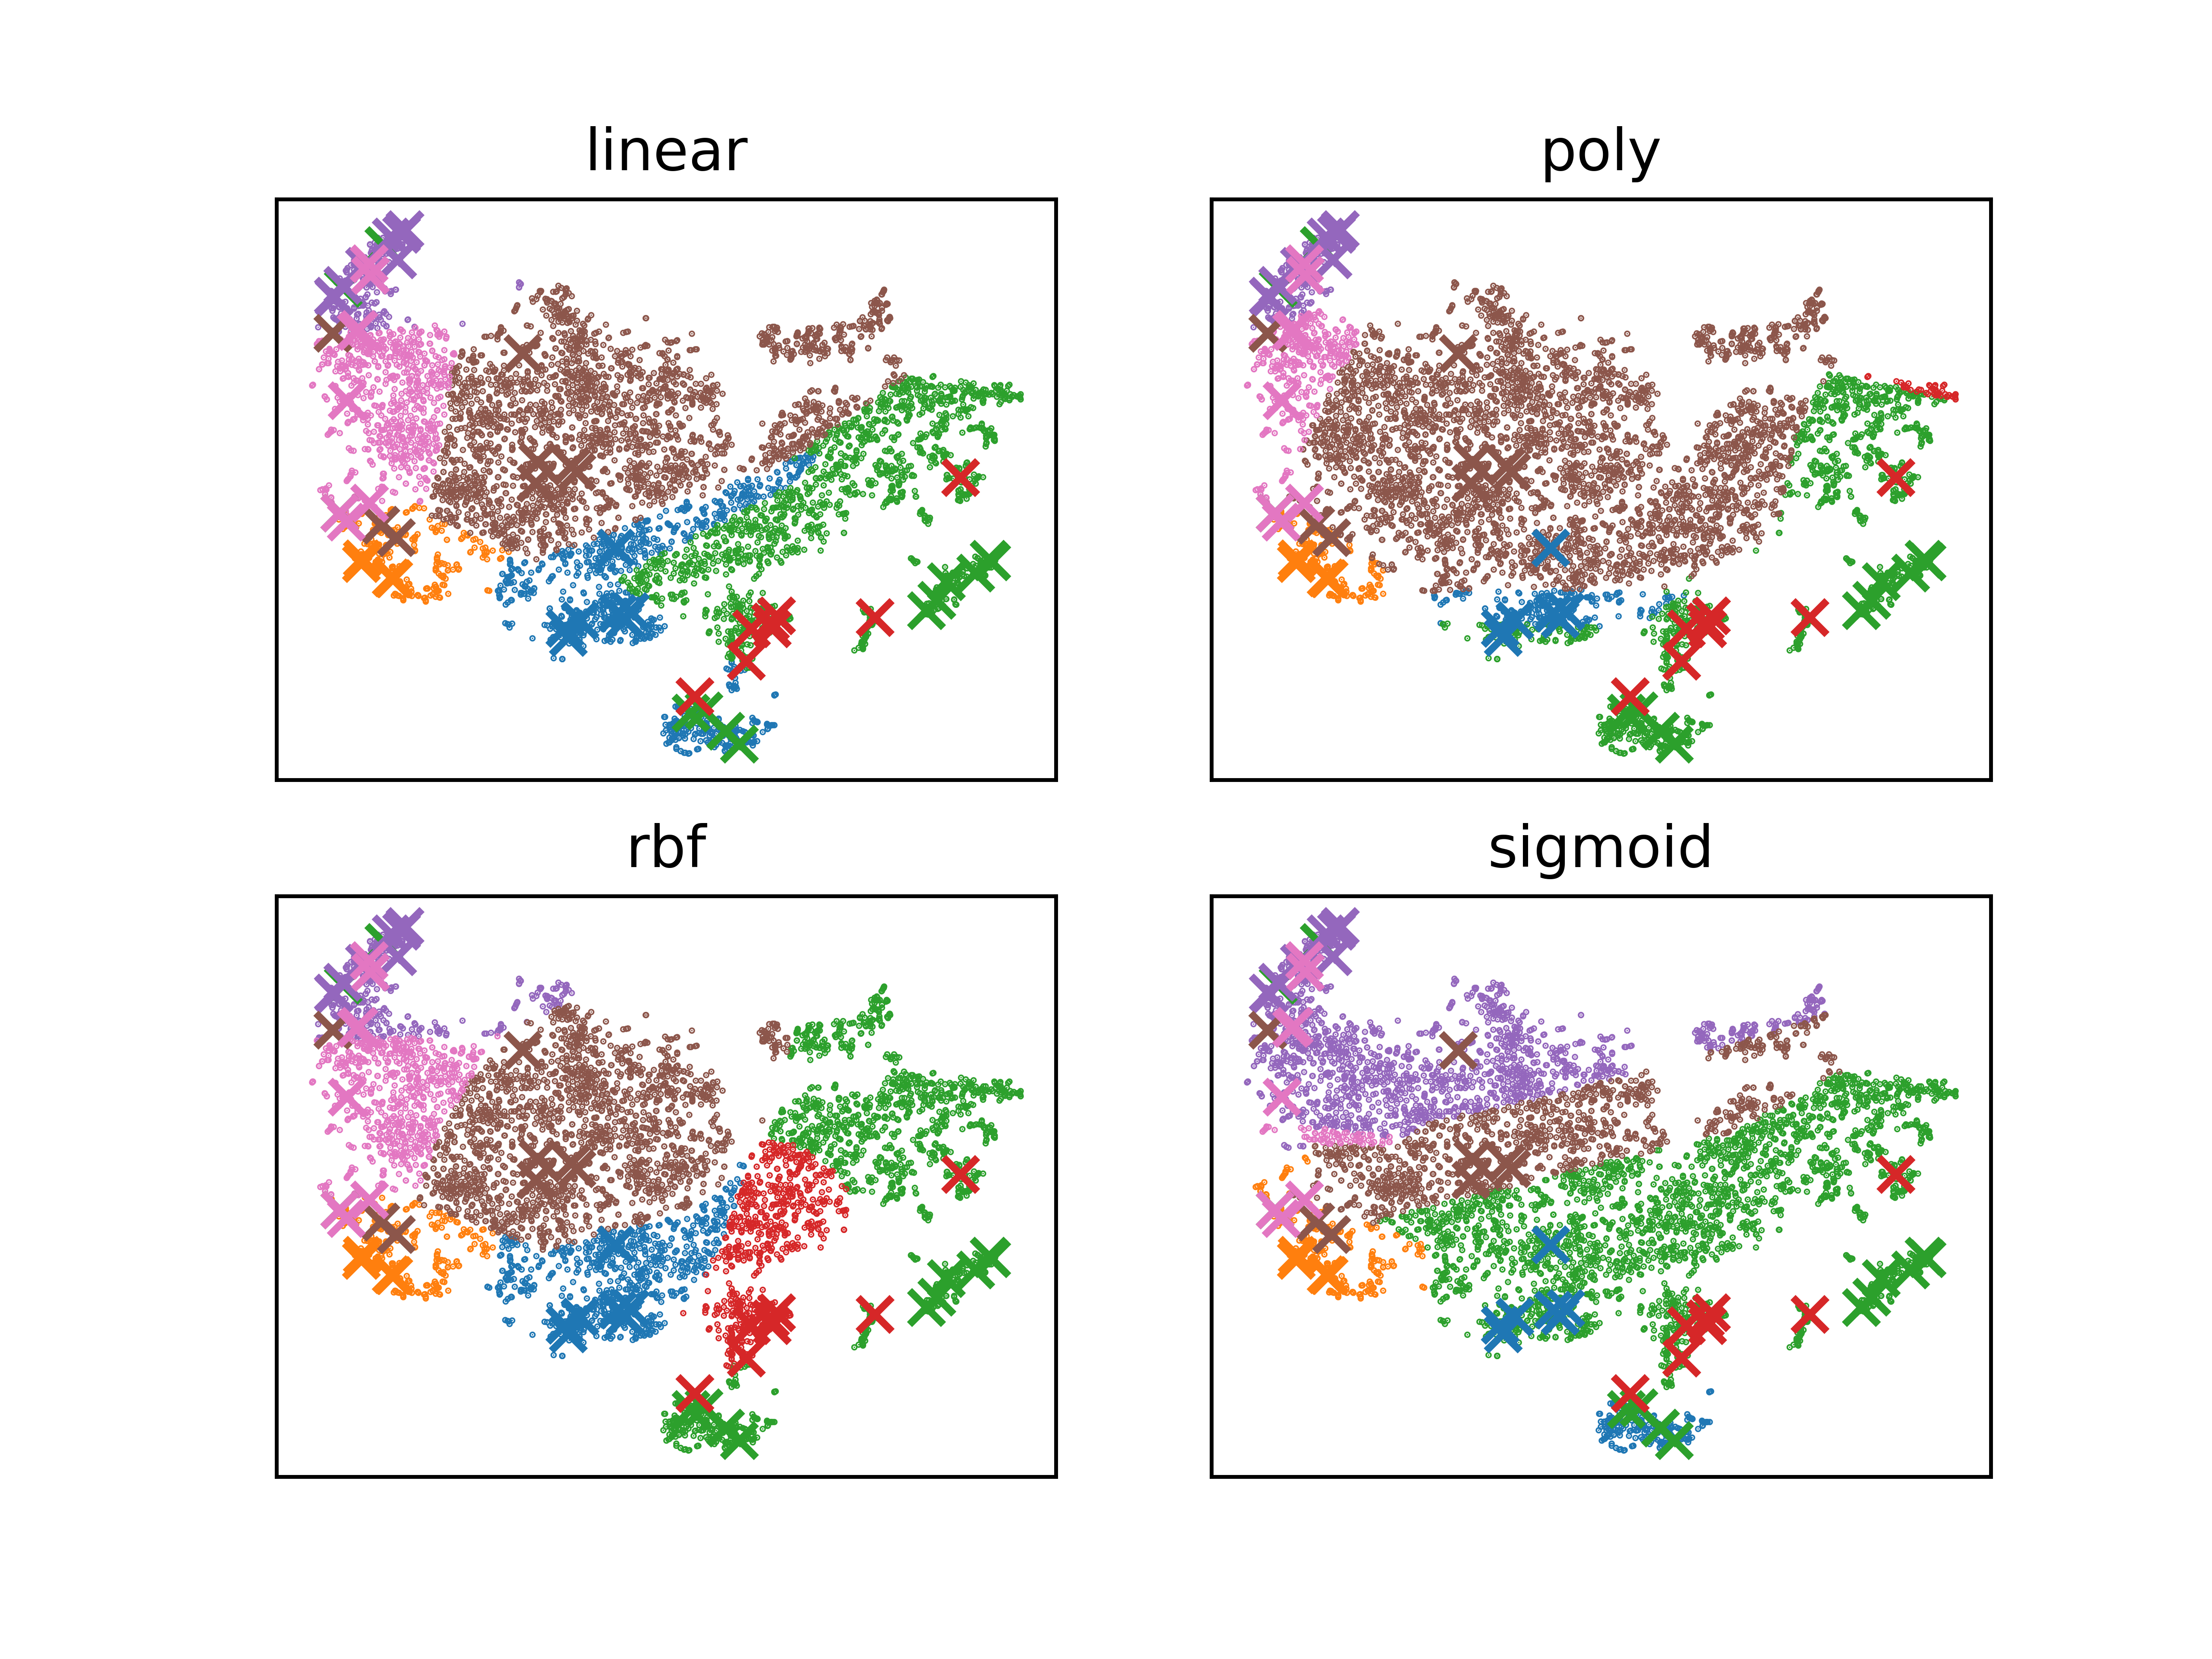
\includegraphics[width=\linewidth]{plots/svc.png}
\end{subfigure}
\caption{Classification with SVC. The kernel specific parameters were left at default.}
\label{fig:svc}
\end{figure}

Now let us move to the (for me) truly novel methods - the decision trees. We will use Gini impurity to decide the splits (Entropy would behave similarly) and the only limitation given is the max tree depth, which is our regularization of the method. The results are seen on Figure \ref{fig:tree}. The results look surprisingly good, however it is known that a single decision tree on its own is not a good estimator - for higher depths (that look very well here), the method has likely overfit. Since we do not have more data available we should use one of the lower depth results to be on a safer side. I should mention that one of the benefits of using a single decision tree is that the results obtained are explainable, since we can always check the tree and the conditions that lead us to each leaf.

\begin{figure}[H]
\centering
\begin{subfigure}{.7\textwidth}
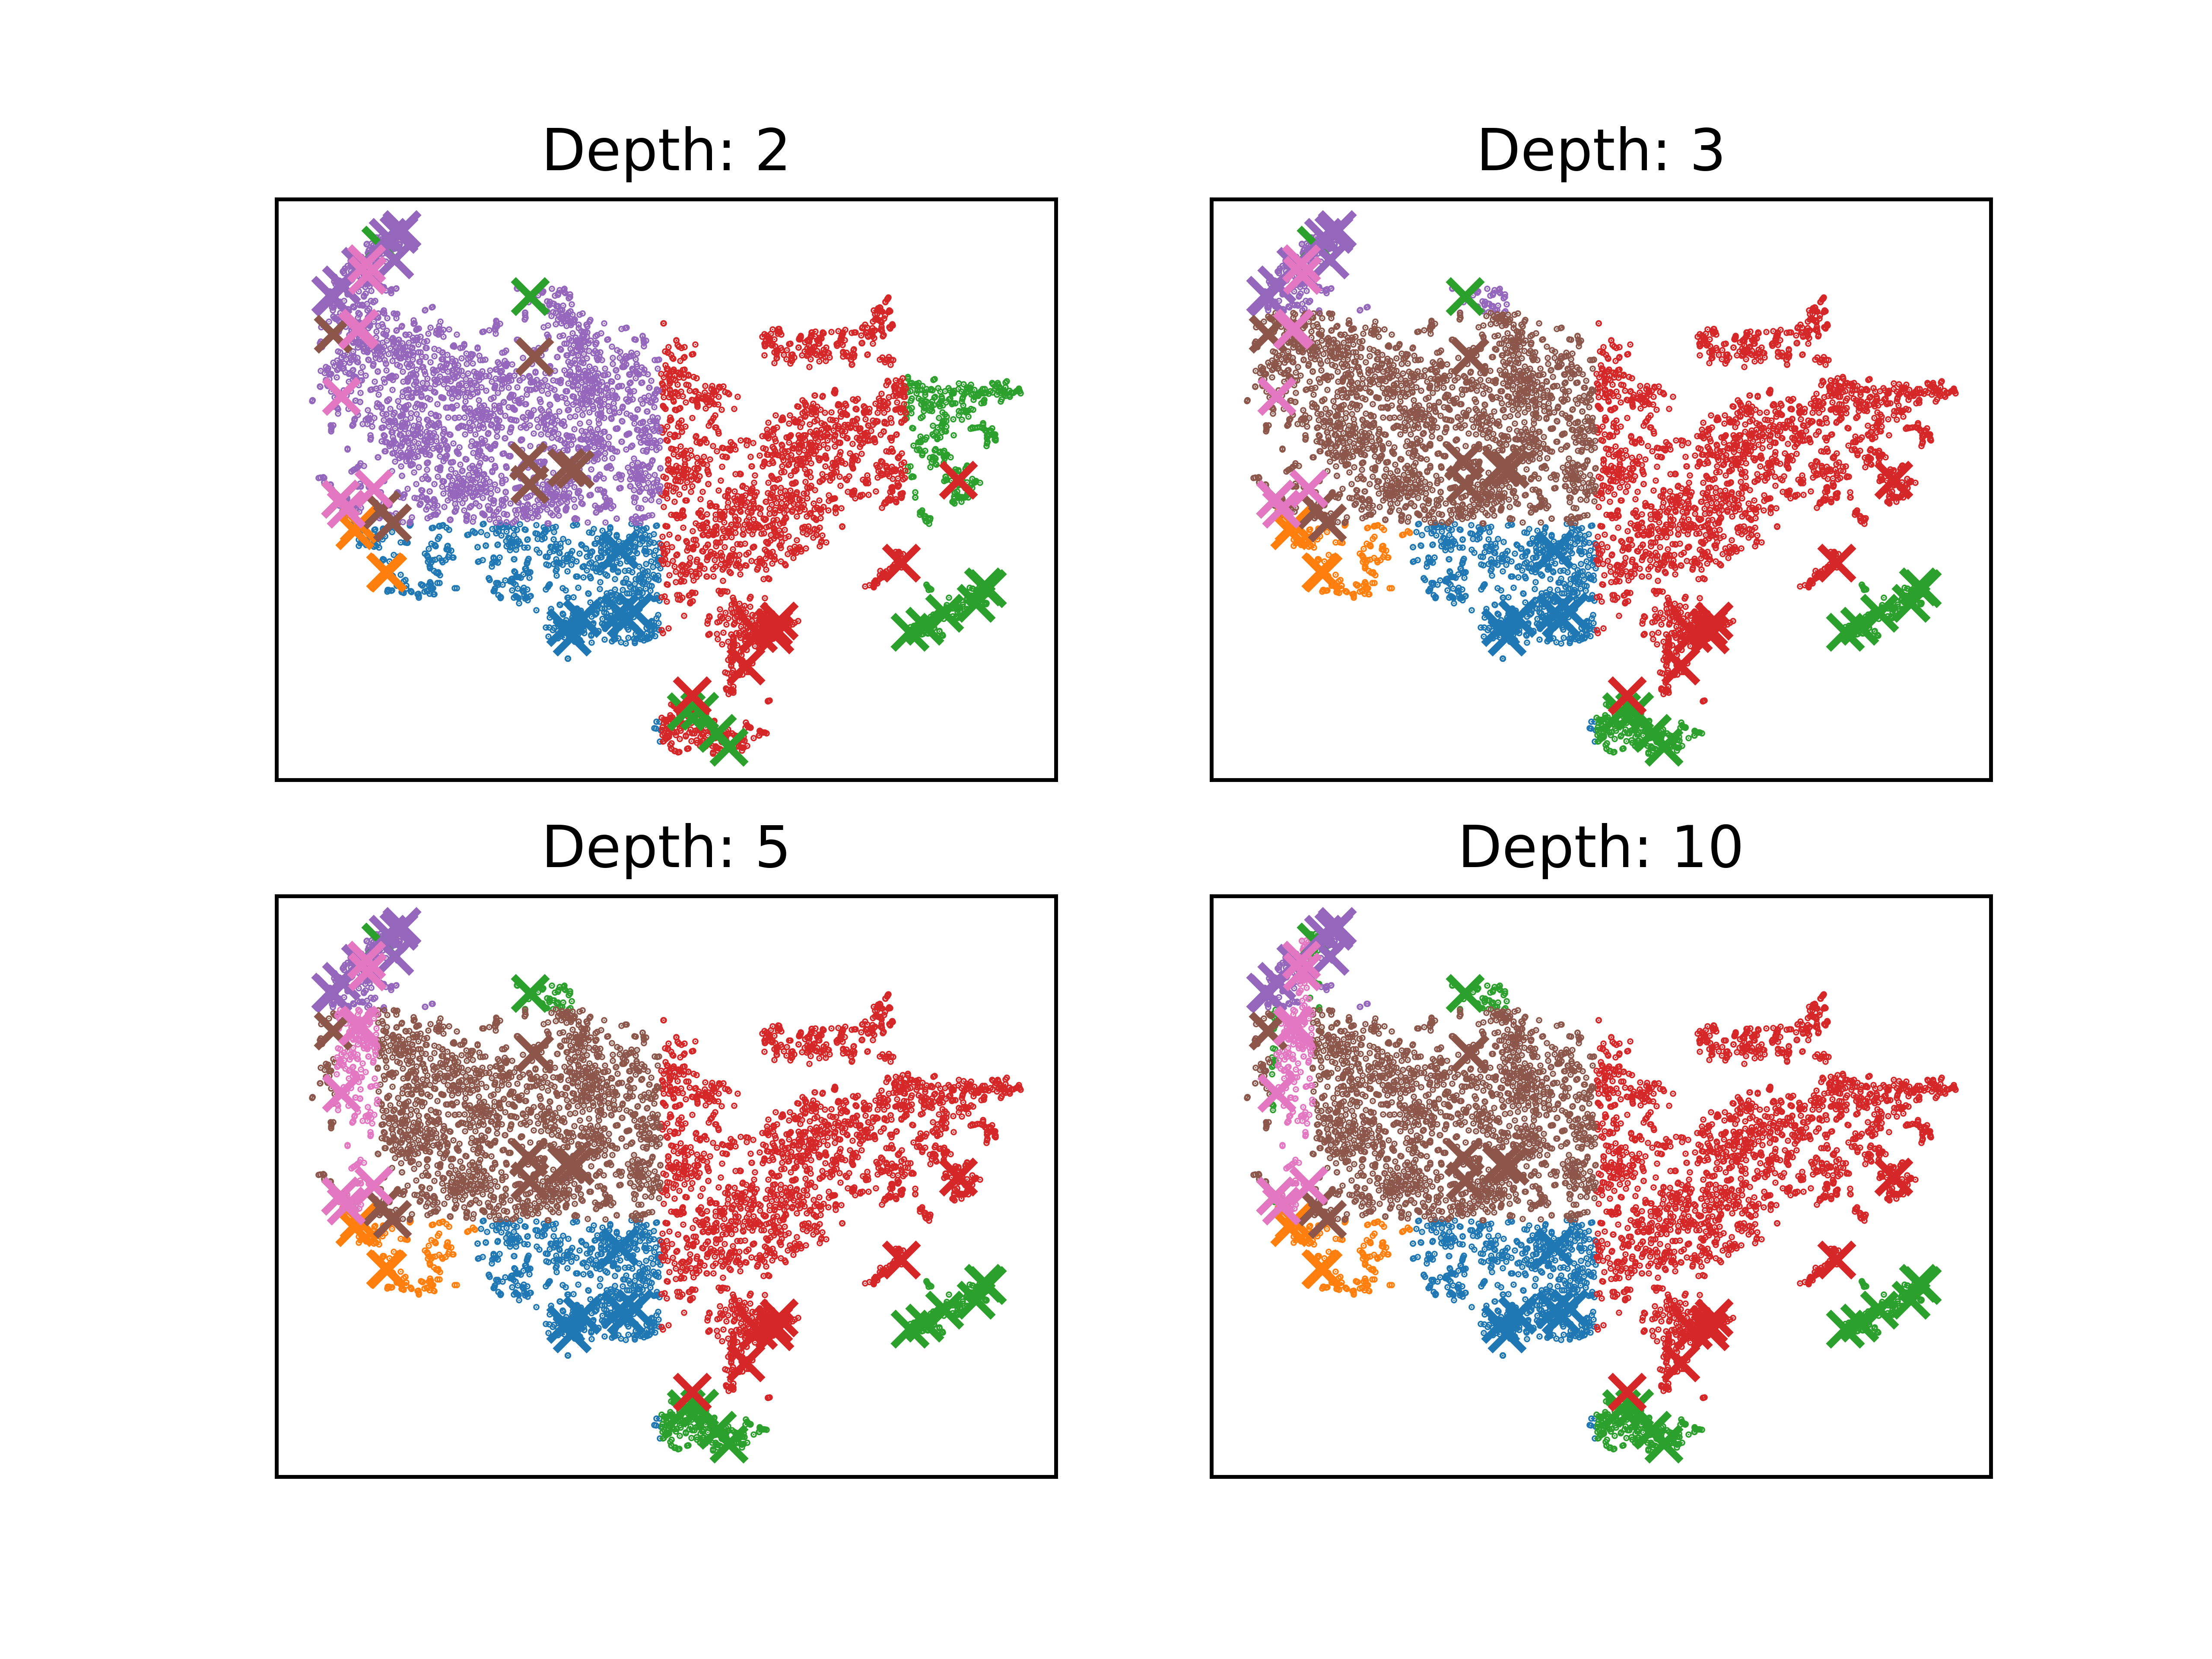
\includegraphics[width=\linewidth]{plots/tree.png}
\end{subfigure}
\caption{Classification with Decision Trees with a certain max depth.}
\label{fig:tree}
\end{figure}

Alternatively, to reduce the risk of overfitting we can use some sort of an ensamble method, which is actually used alot more comonly in practice. We use gradient boosted trees, which is shown on Figure \ref{fig:gradTree}. We've only changed the max depth and number of estimators (trees) parameters, the other parameters are well dependent on these two anyway. Learning from our previous experience with a single decision tree, the depth parameter allows the method to perfectly fit very quickly, so we set that parameter very low in the ensemble method (the point is to use alot of weak classifiers). The results look well even already for trees of depth $1$.

\begin{figure}[H]
\centering
\begin{subfigure}{.7\textwidth}
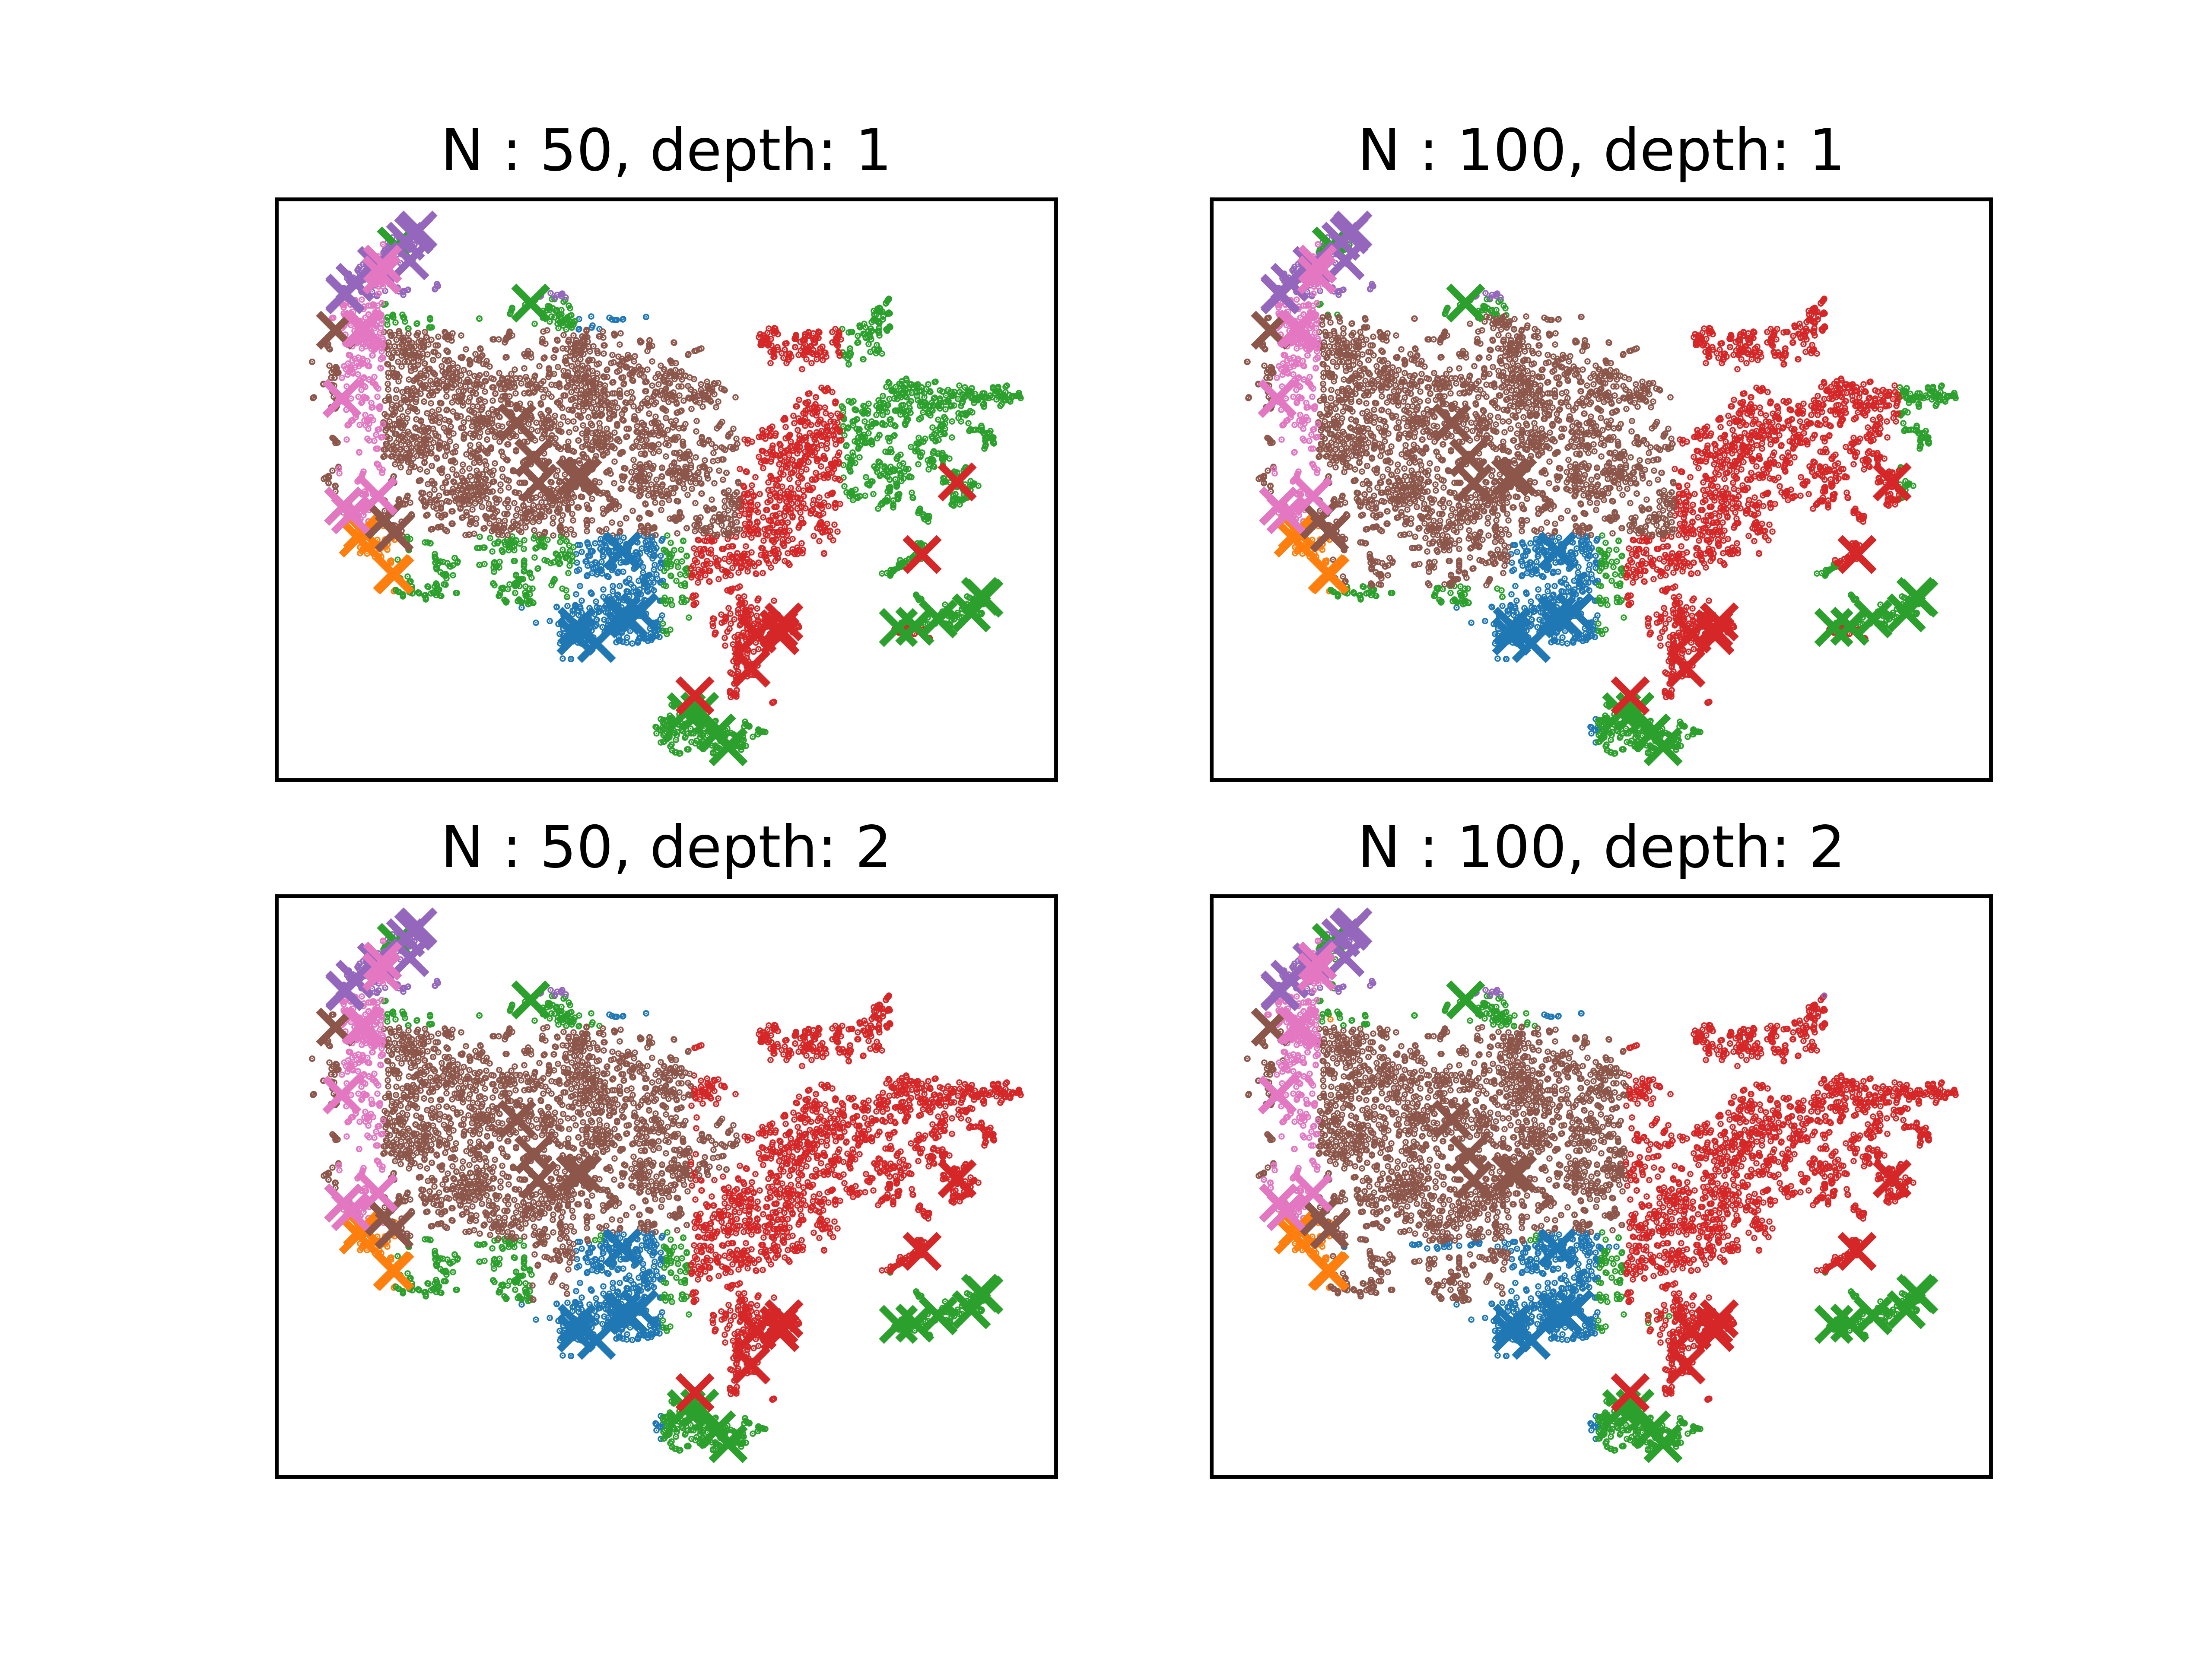
\includegraphics[width=\linewidth]{plots/gradTree.png}
\end{subfigure}
\caption{Classification with boosted decision trees with a certain number of classifiers (N) and max depth.}
\label{fig:gradTree}
\end{figure}

Let's try another ensemble method - random forests, where different trees are built from the data using bootstrapping and than collectively used to obtain the classification. The results can be seen on Figure \ref{fig:randomForest}. The depth 1 results seem to inherit the bad properties of the single decision trees, which is unable to classify the red crosses. The depth 2 cases look much better. Alternatively, the max features parameter of the decision trees could be changed (now it was set to its default value) to allow for more flexibility even at a depth of 1. 

\begin{figure}[H]
\centering
\begin{subfigure}{.7\textwidth}
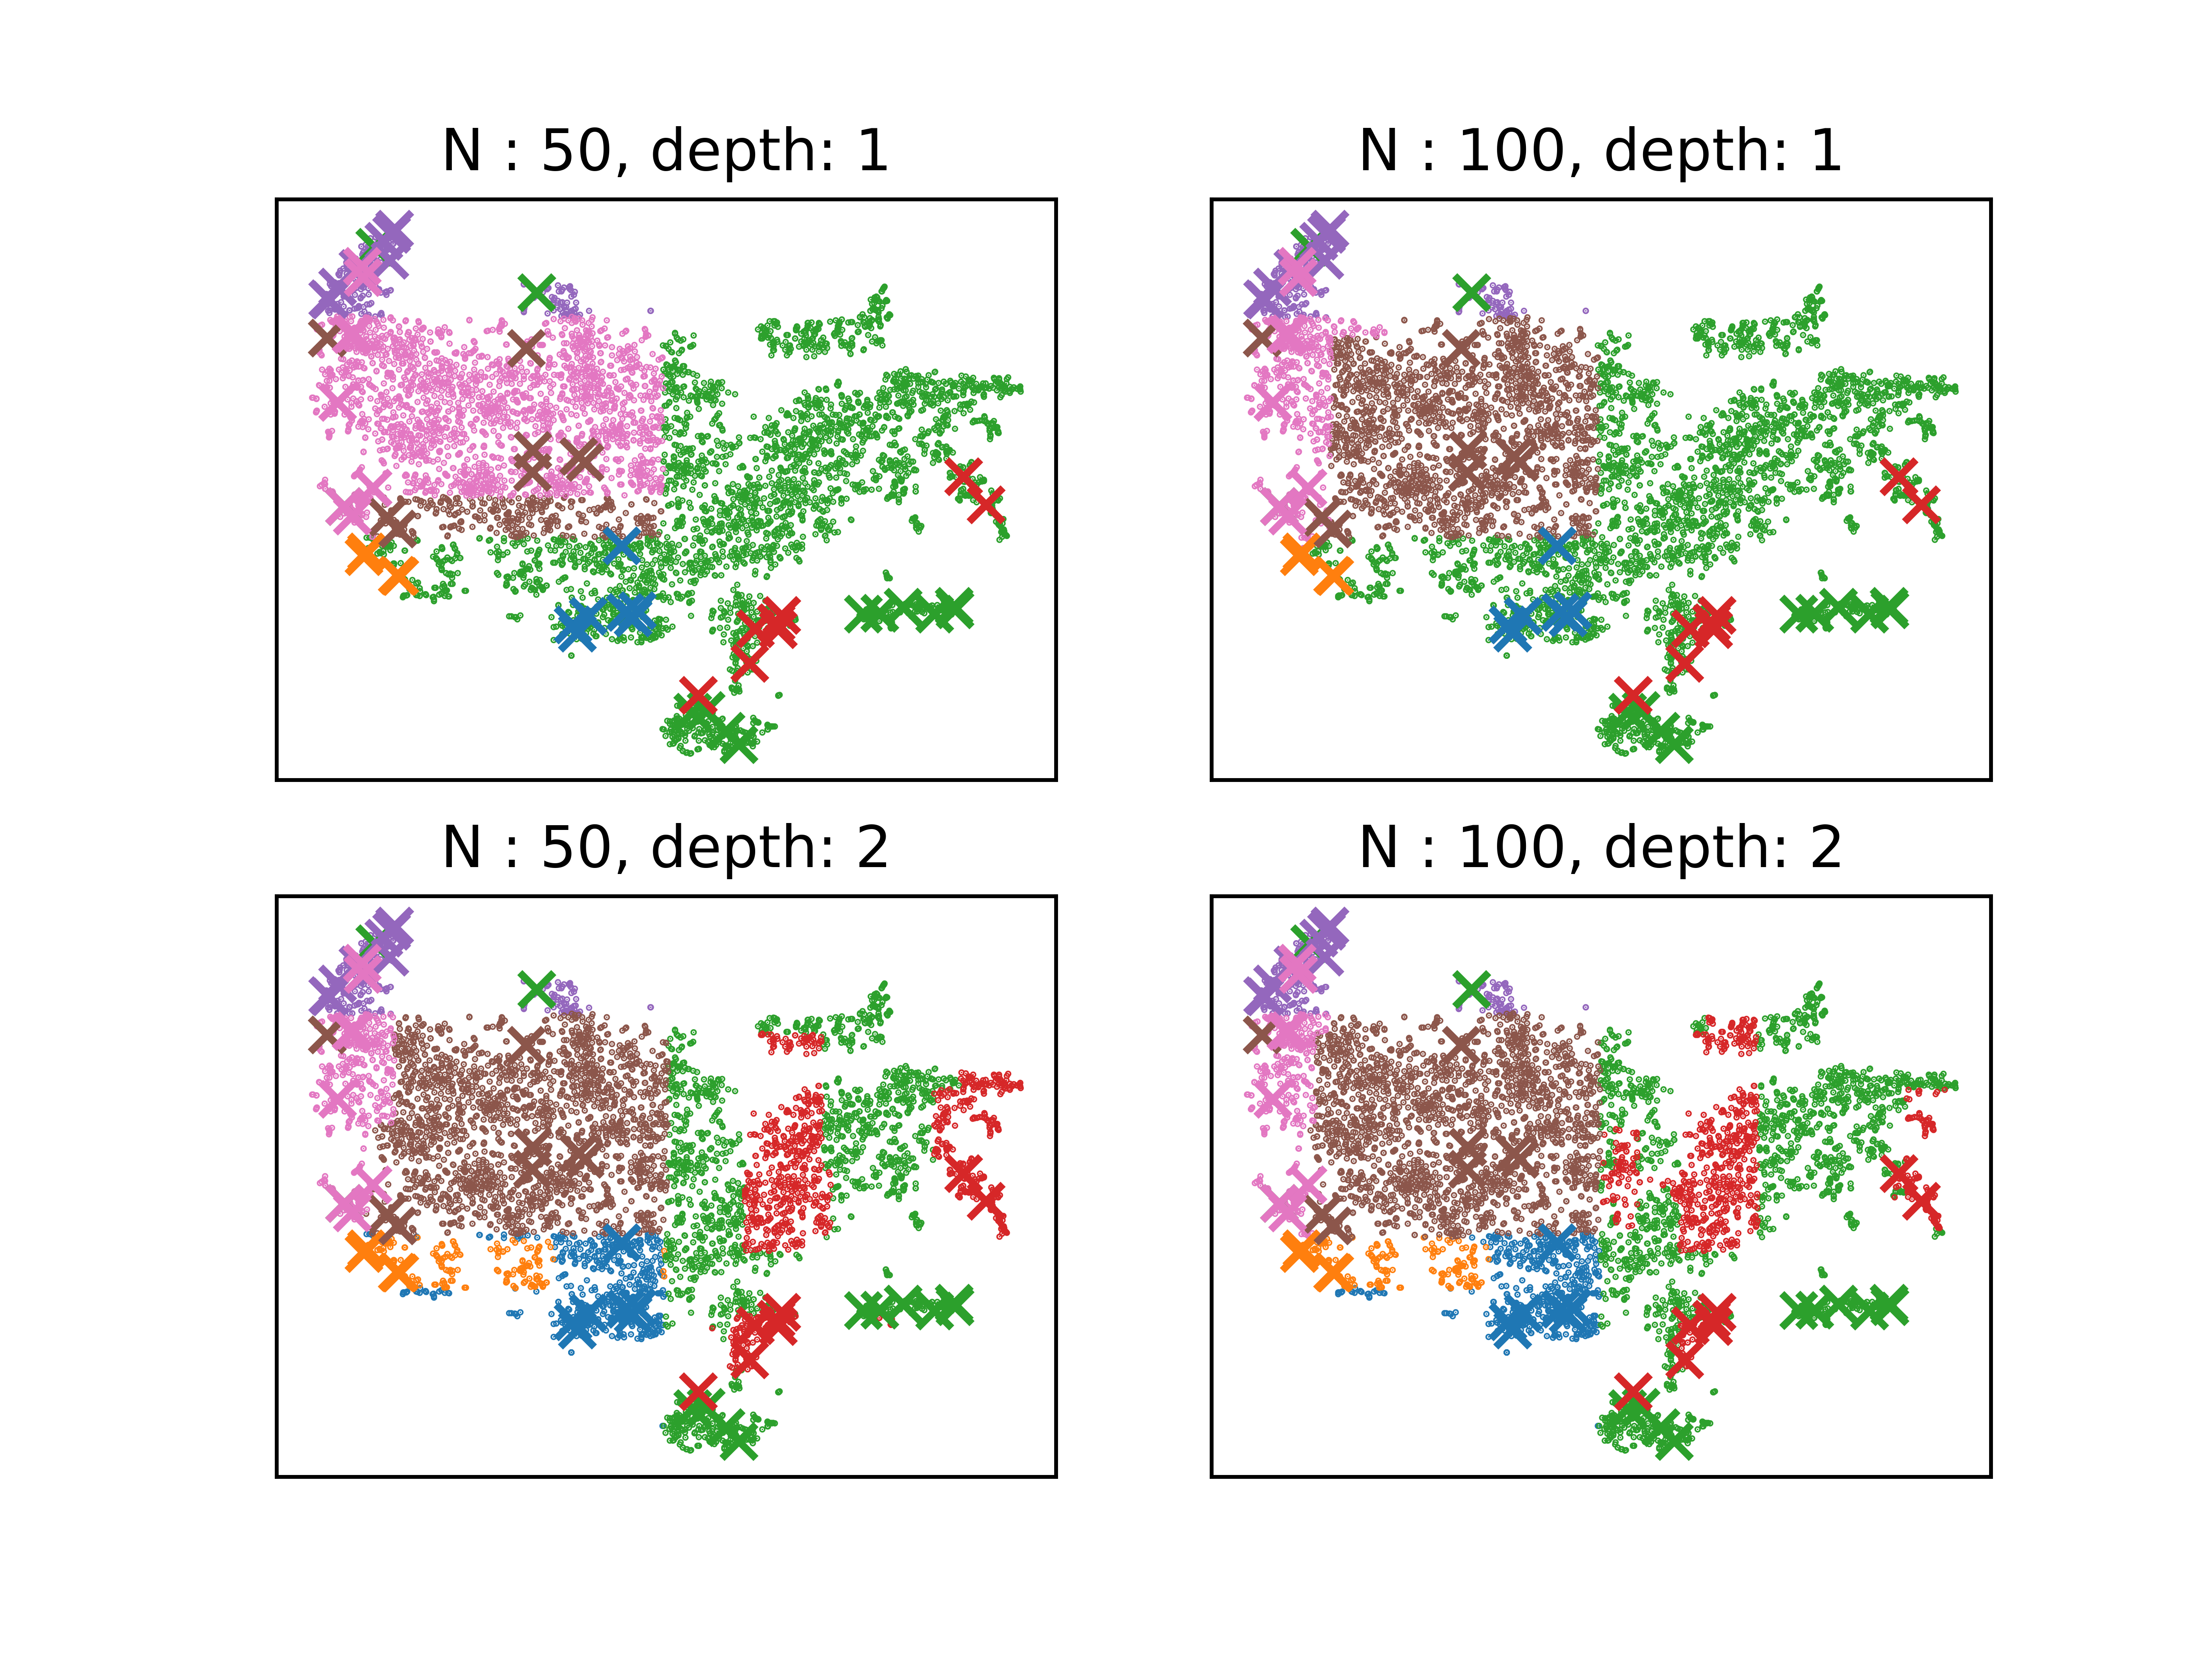
\includegraphics[width=\linewidth]{plots/randomTree.png}
\end{subfigure}
\caption{Classification with random forests with a certain number of classifiers (N) and max depth.}
\label{fig:randomForest}
\end{figure}

Lastly, let us resort to Gassian naive Bayes, where Bayes' theorem is once again used, with priors given simply as fractions from labeled data and the distribution of data (conditioned on a certain class label) is independent of other data. Figure \ref{fig:nb} shows the result of such a classification method. Very weirldy, some of the points in the right of the figure have been deteced as belonging to the orange (TRI) specter.

\begin{figure}[H]
\centering
\begin{subfigure}{.7\textwidth}
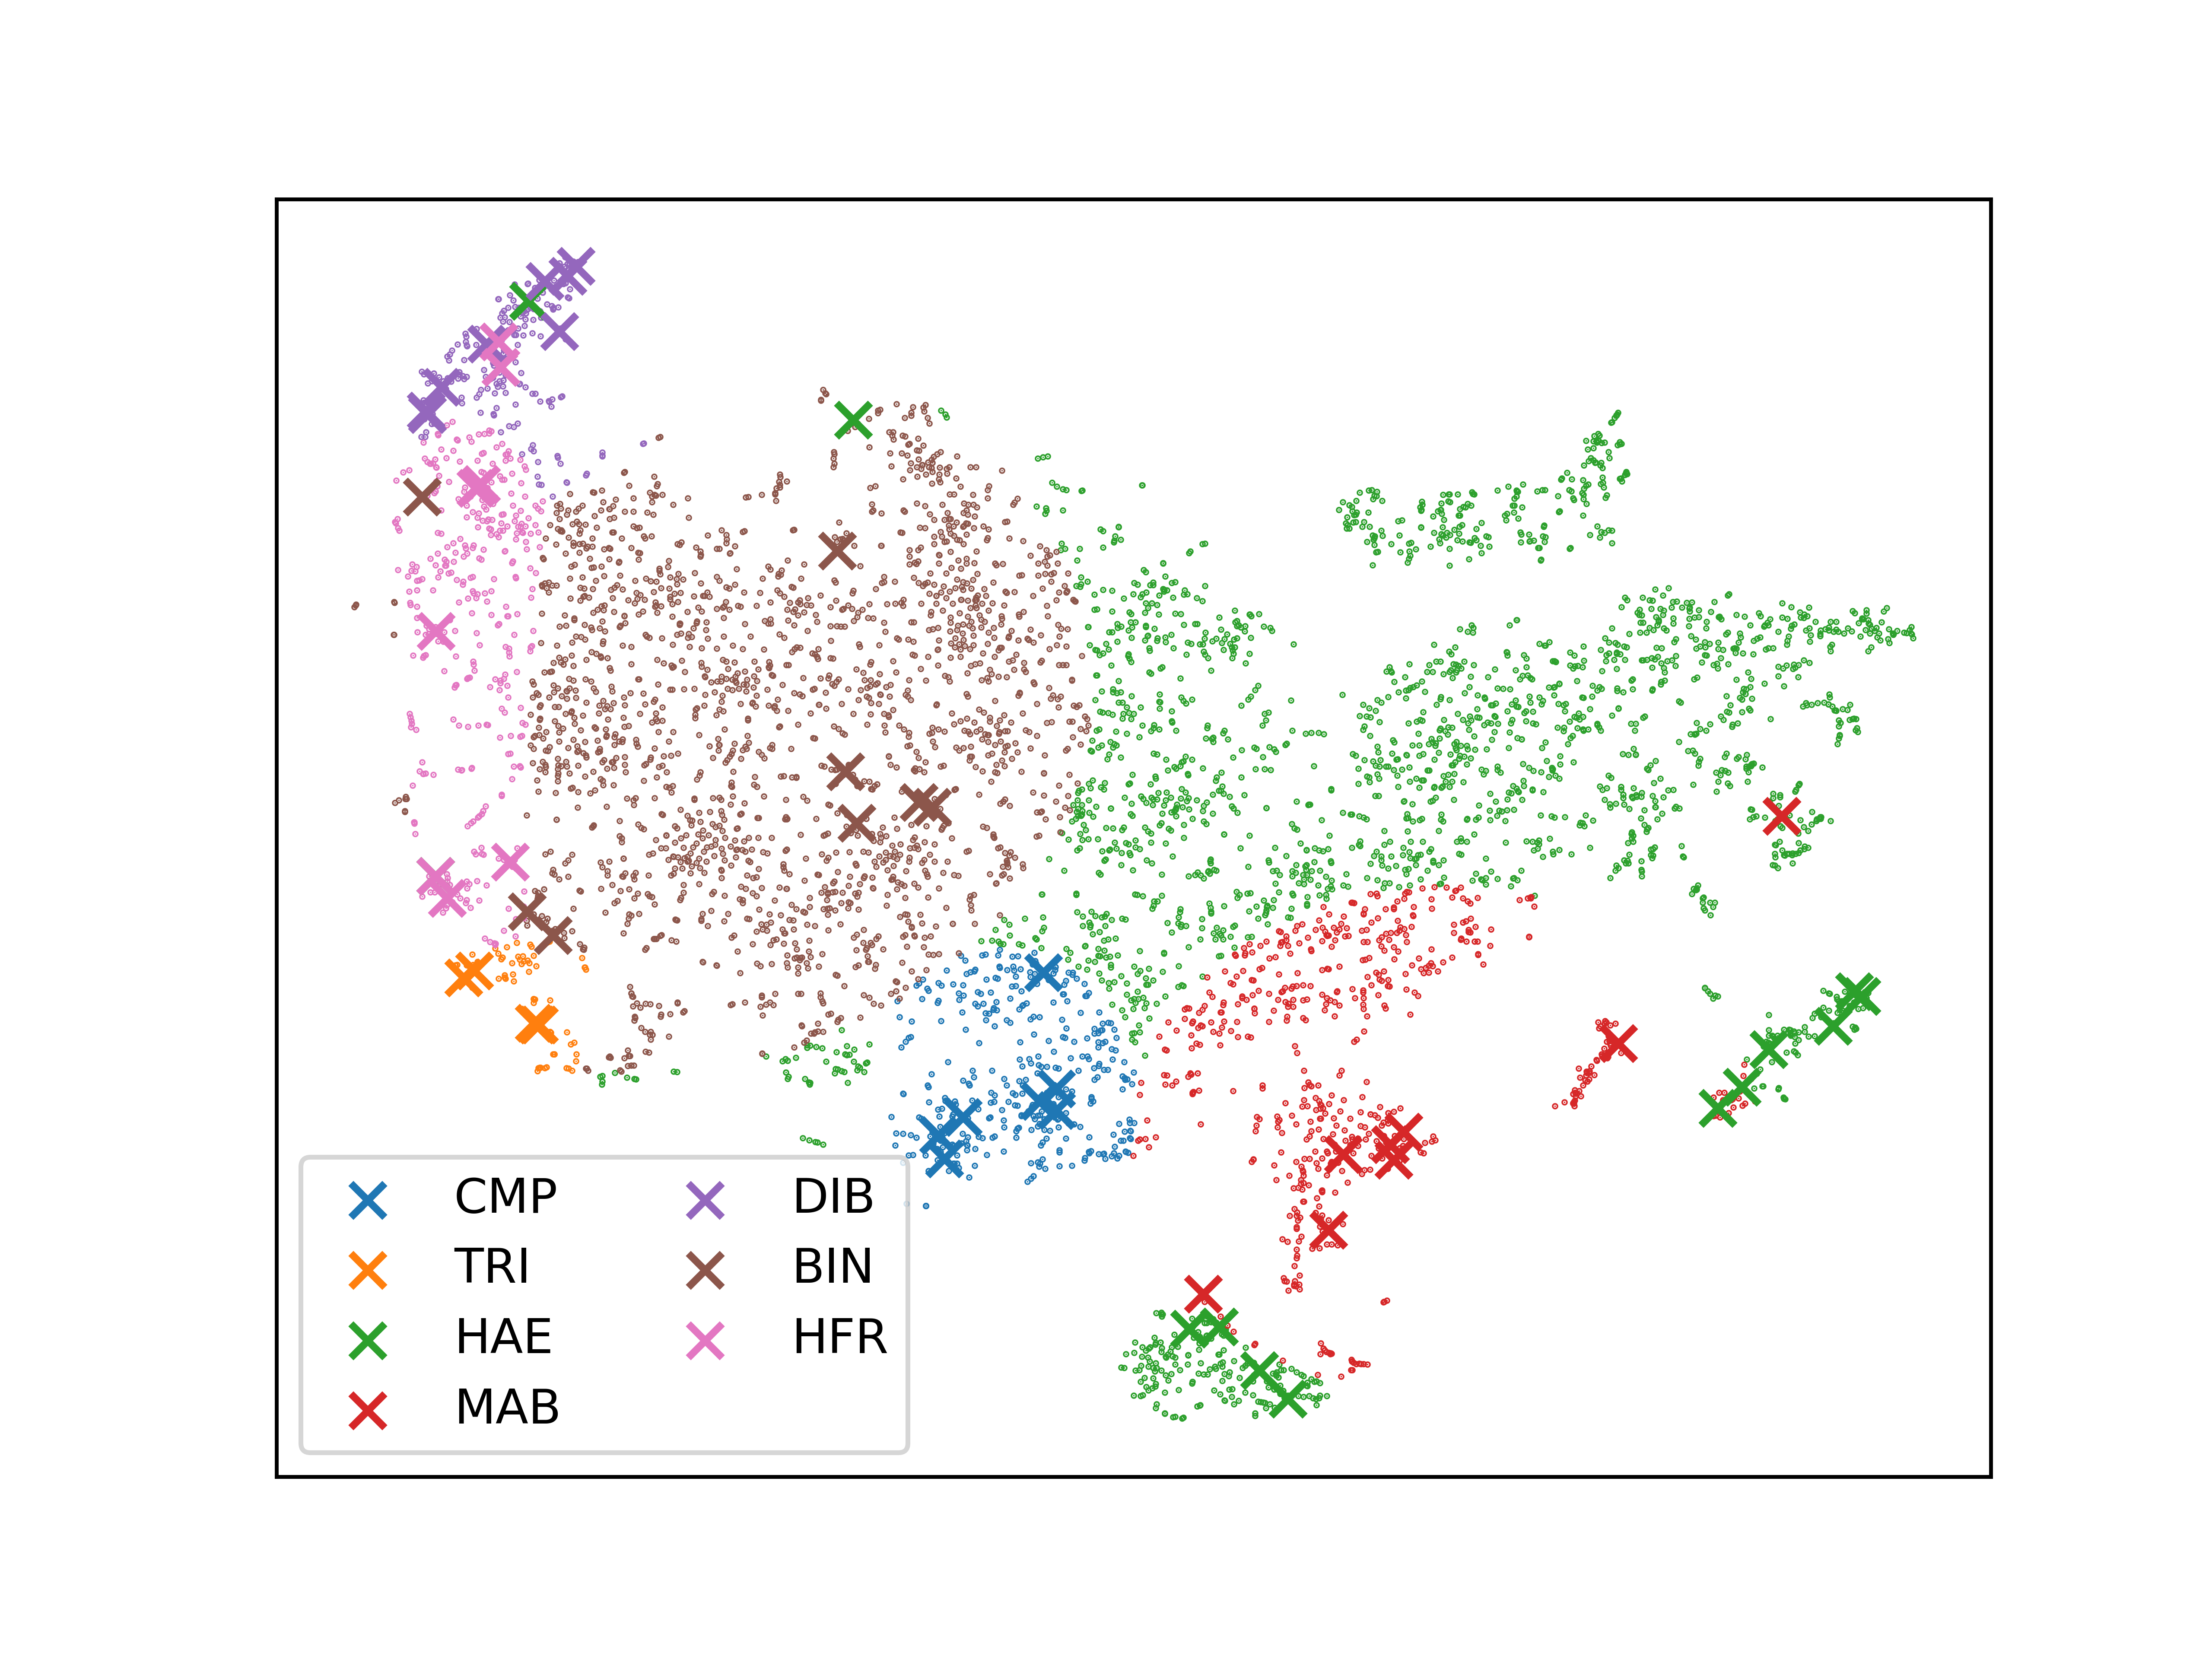
\includegraphics[width=\linewidth]{plots/nb.png}
\end{subfigure}
\caption{Classification with Gaussian naive bayes}
\label{fig:nb}
\end{figure}

\section*{Conclusion}
In the dimensionality reduction step, clearly RBF Kernel PCA and tSNE fared the best. After the projection we could immediately (visually) classify some unknown spectra as belonging to a specific class, but a big amount are a big distance from any labeled spectra and thus more difficult to classify.

We have tried a number of classifiers without a clear winner. 
We have not performed some common tricks for cross-validation in part because the amount of training data was so low, but also because we are leaving this aspect of ML for future projects. While this would definitely help with improving our results, working with what we have done, it seems that the safest classifier would be one of the more simple ones, as we do not have enough data to support a complex model (also, Occam's razor). Perhaps I would go with the cubic logistic regression, as it is not a very difficult algorithm, while still giving visually sensible results.
\end{document}
